\chapter{\java{} Applications on SGX}
\label{chap:civet}


\newcommand{\sysname}{Civet}
\newcommand{\jvm}{JVM}
\newcommand{\jvmname}{OpenJDK 7}
\newcommand{\staticphase}{design-time}
\newcommand{\statictool}{Shredder}
\newcommand{\dynamicphase}{execution-time}
%\newcommand{\dynamicframework}{Escalator}
\newcommand{\dynamicframework}{Connector}
\newcommand{\tcbsize}{trusted code size}


\makeatletter
\newcommand{\Capitalize}[1]{%
	\edef\@tempa{\expandafter\@gobble\string#1}%
	\edef\@tempb{\expandafter\@car\@tempa\@nil}%
	\edef\@tempa{\expandafter\@cdr\@tempa\@nil}%
	\uppercase\expandafter{\expandafter\def\expandafter\@tempb\expandafter{\@tempb}}%
	\@namedef{\@tempb\@tempa}{\expandafter\MakeUppercase\expandafter{#1}}}
\makeatother

\Capitalize{\dynamicphase}
\Capitalize{\staticphase}


\makeatletter
\def\input@path{{civet/}}
\makeatother
\graphicspath{{civet/figures/}}

\begin{abstract}

  Application partitioning is a technique to move sensitive data or code into
  a protected environment, such as an SGX enclave.
  Partitioning larger existing applications requires subtle reasoning that can be aided with static
  analysis and dynamic, language-level techniques.
  For instance, in-enclave code may include a library that memoizes results in the out-of-enclave heap.
  Using a managed, type-safe language like Java in SGX also brings the benefits of partitioning to a large body of 
  existing code. %, as well as help the developer with language-level analysis tools.
  Unfortunately, running Java partitions in SGX introduces a number of technical
  challenges, many of which arise from resource and system ABI constraints.
  To our knowledge, no prior work has even run a complete Java application in an enclave,
  much less partitioned a Java application to run a piece of application logic in the enclave.
%  That said, no amount of application-level analysis can protect against
%  a compromised OS, without 
  Thus, a number of technical challenges must be addressed to unlock
  the benefit to developers of combining managed languages with hardware such as SGX.


%% \fixmets{Streamlined the argument for combining Java and SGX. Check if this makes sense.}
%% %%There have been significant, but separated %often mutually exclusive,
%% There have been significant, but often mutually exclusive
%% advances in hardware and language-level tools for partitioning applications
%% into multiple security contexts or privilege levels.
%% %Developers who build security-sensitive applications
%% %often face the dilemma of choosing between
%% %managed language features and hardware protections with language restrictions.
%% Developers either 
%% use a hardware solution, such as \intel{} \sgx{},
%% to isolate a piece of consolidated code %small piece of native binary code
%% from an untrusted OS, %but the developer
%% %must reason carefully about potential information flows that could leak data from the enclave, as well as other vulnerabilities in the code.
%% %On the other hand, in
%% or choose to program in a managed type-safe language, such as Java, 
%% %the developer has 
%% which has a wealth of tools and properties for 
%% improving code security and application partitioning.
%% %from type-checking to 
%% %more advanced tools to secure control and information flows.
%% The use of hardware
%% and language-level tools for partitioning are often complementary by concept but incompatible in reality.
%% %mutually exclusive,
%% %due to the limitations in combining the technologies.
%% %This paper observes that these language and hardware security tools 
%% %should complement each other, but are often mutually exclusive.
%% For instance, no language-level analysis %of an application
%% can protect an application against a compromised OS.
%% However, it is fundamentally challenging to
%% factor the protection of \sgx{} into the analysis of a managed type-safe language like \java{}.
%Running a managed language in an enclave is difficult, and language tools
%currently do not factor the hardware capabilities of \sgx{} or similar hardware into their analyses.


%Similarly, the \sgx{} hardware imposes restrictions on loading \java{} classes 
%with \jvm{}s;
%the \java{} language also lacks sensible APIs for using \sgx{} hardware.
%to wrap the semantic of interfaces with the 

%but are not sufficient to defend against a compromised OS or hypervisor.
%but the developer must partition the application 
%and harden the code inside the enclave.
%Managed languages, such as \java{},
%offer a wealth of language-level support for 
%but are not sufficient to defend against a compromised OS or hypervisor.
%The two approaches are often mutually-exclusive:
%we are unaware of any prior work thas has run a \jvm{} inside of an enclave at all,
%For \sgx{} and \java{},
%there is no prior work that has run a \jvm{} inside an enclave,
%much less integrated enclaves into the language's analysis tools.
%\fixmedp{check my claim. Too strong, or justified?}
%\fixmets{Since we are generalizing, we should only claim this is the case for sgx vs. Java. BTW, I prefer showing more certainty when making claims.}


%Application developers can place a library and sensitive data
%in an \intel{} \sgx{} enclave,
%but only if the library is a native binary, generally written in C.
%but must relies on developers to design invulnerable code.

%more advanced tools for detecting information flows.

%These language-level tools can be invaluable in ensuring a correct application partitioning
%and overall application correctness.
%Unfortunately, the most security-sensitive developers must choose between
%hardware and language security tools.


%% Using \intel{} \sgx{} enclaves, applications can
%% protect their most critical components from untrusted system stacks.
%% Language support for \sgx{} enclaves is a missing feature of existing \java{} Virtual Machines.
%% Using a managed language like \java{}
%% provides an opportunity to improve the weakest link of the enclave security---
%% application vulnerabilities that lead to information leakage.
%% \java{} language has effective framework to trace information flows, and provides type safety
%% to prevent memory access vulnerabilities in the enclave.
%% In addition, modularization in \java{} classes allows automatically partitioning
%% an application into enclave components,
%% minimizing the classes included in the enclave's trusted computing base.

This paper presents {\em \sysname{}},
a system that integrates \java{} language tools for partitioning applications
with run-time support for isolated execution in \sgx{} enclaves.
%\fixmedp{Any reason we can't do more than one partition in the enclave?}
%\fixmets{For an application, there is only one partition: the secure-sensitive part. We can create more than one instances in an enclave.}
%and which can execute a portion of the \java{} application in 
%a \java{} utility, runtime framework and API,
%that helps developers design isolated application components,
%and minimizes the attack vectors.
\sysname{} includes both \staticphase{} and \dynamicphase{} components.
The \staticphase{} tool, {\em \statictool{}}, uses code reachability analysis
to determine the minimal required \java{} classes for the isolated execution,
and helps the developer understand the complete partition interface. % between the application partitions.
%\sysname{} helps the developers generate an enclave image
%with minimal required \java{} classes for the protected code, reducing the TCB. %required for isolated execution.
%%\sysname{} includes language-level information flow control at the 
%%enclave border, protecting against unexpected exfiltration of secret
%%data due to application vulnerabilities.
The \dynamicphase{} framework, {\em \dynamicframework{}}, then launches the isolated execution of the enclave image
(a signed JAR archive) in an enclave when the untrusted part calls the interface.
Throughout the execution, \sysname{} enforces end-to-end isolation
on any object instantiated inside the enclave,
and leverages language-level information flow control to determine whether an object contains no sensitive information before the object is released from the enclave.
%to protect against unexpected ex-filtration of secret
%data. % due to application vulnerabilities.
%\fixmebj{How about this?}
%\fixmedp{Is this best-effort?  Only for explicit flows?  The 
%preceding sentence should be crisper}
%identifies information flow at the enclave border,
%preventing enclave secrets
%from being leaked due to any vulnerabilities.
%with minimal classes needed for the isolated computation,
%and narrowest interface for interaction.
%Second, the framework effectively prevents information leakage
%by forbidding any objects tainted by information flow to leave the enclave.
%In \sysname{},
%trusted servers may provision secure objects and classes,
%preserving security policy information. \fixmedp{Don't understand the previous sentence}
%\fixmedp{Do we want to say anything about contributing techniques to get good performance?}
%To secure \java{} applications, 
%With both the \staticphase{} and \dynamicphase{} language support,
\sysname{} also creates language-level abstractions of and extensions \sgx{},
such as attestation and provisioning, simplifying cumbersome aspects of this hardware
for developers.
%extends the security properties (e.g., data confidentiality) and features (e.g., attestation and provisioning)
%of \sgx{}, %hardware protection to cover \java{} classes dynamically loaded by the \jvm{},
%and encapsulates cumbersome aspects of interfacing with the hardware architecture
%keeps the work of bootstrapping and interfacing with 
%from application developers.
%As a proof-of-concept of using advanced language-level tools,
%we use \sysname{} %strengthens hardware protection
%to identify and remove 
%by filtering 
%implicit information flows that would leak secrets from an enclave
 % that leaks secrets
%in our test applications.
%\fixmedp{all of them?  Or just one?}\fixmets{I think this technique applies to all test cases.} % error-prone applications. 
%Finally, the API allows components in enclaves to be seamlessly provisioned with
%secure objects or classes by trusted servers,
%and to preserve their security policy information.
%with security guarantees extended from their sources.
%\sysname{} is evaluated with \jvmname{} on the latest 
%We evaluate \sysname{} % with several case studies 
%on the latest \intel{} Skylake processor.
%Evaluation shows good performance on
%Our overheads are low, 
%adding \fixmedp{xx}\% overhead on an isolated cryptographic library used in SSH client/server,
%and \fixmedp{xx}\% overhead on Hadoop jobs that run a secret, provisioned algorithm.
We demonstrate the usage of \sysname{} with two applications: a SSH server with an isolated cryptographic library to protect its host key,
and a Hadoop framework capable of securely executing jobs using any secret, provisioned algorithm.
%\sysname{} reduces the developer effort required to partition the application code,
%resulting in a smaller 
%and the result of integration is highly generalizable to other managed languages.
%~\fixmebj{Always replace TCB with code footprint size to indicate that we are only talking about size of code - not attack vectors.}
%\fixmets{find a better term for TCB size}
%~\fixmebj{Always replace managed languages with managed type-safe languages.}
%\fixmets{accurately separate managed language and type-safety: managed language causes the challenges, and type-safety improves the security properties; Java happens to be both.
%}
\end{abstract}

This chapter describes the formal definition of the \graphene{} host ABI.

\section{Basic Definitions}

The \graphene{} host ABI defines a set of {\em functions}, similar to the API of UNIX or POSIX.
The functions are directly called by the library OS, along with the arguments given either in the registers or on the stack.
A host-specific \graphene{} loader is responsible for resolving the linking, from the library OS to the host ABI.
%\papersection{Challenges for Partitioning with Enclaves}
\label{sec:background}
In this section, we will give a brief overview of \sgx{}, and discuss 
the key challenges developers face when trying to manually partition applications using a technology such as \sgx{}.
%discuss the programming models and threats to security of \sgx{} enclaves.

\papersubsection{Background on \intel{} \sgx{} Enclaves}

\intel{} \sgx{} ({\it Software Guard Extension})
is a set of new x86/x64 instructions
introduced in the \intel{} Skylake processor family.
Using \sgx{}, an 
application can designate part of its virtual memory as an {\em enclave}.
The CPU guarantees that the contents of the enclave never leave the CPU package unencrypted.
The CPU also measures the integrity of a binary loaded into the enclave, and offers remote attestation,
similar to a TPM\fixmedp{cite}.

%%% create a protected memory region, called an {\em enclave}, inside it's virtual memory,
%%% where it can load its security sensitive data with hardware-enforced isolation from the untrusted OS. 
%%% The processor with \sgx{}
%%% guarantees that any data loaded in enclave
%%% stays encrypted in the DRAM, by using a secret key deterministically derived from the application's cryptographic measurement and the CPU secret. 

\sgx{} is an appealing tool for protecting small amounts of highly-sensitive data or code, because it can defend 
against a malicious or compromsed OS, hypervisor, or even hardware peripheral.
For instance, \fixmedp{Foo} et al.~\fixmedp{cite that \sgx{} workshop paper} show how \sgx{} can be used
to build a trusted path from a video chat application to a GPU and network card, which maintains confidentiality and integrity of the
video stream, even if the OS is compromised.
Simlarly, because DRAM contents are encrypted, \sgx{} can resist cold-boot attacks~\cite{halderman09coldboot} or 
malicious peripheral devices~\cite{hudson15thunderstrike}.


%%% \sgx{} also proves the integrity of loaded binaries to remote trusted entities
%%% using mutual attestation based on a symmetric key generated from the measurements of communicating entities.
%%% \sgx{} usage model mostly involve the launched enclave mutually attesting the trusted host
%%% to obtain provisioning of security-sensitive information
%%% through a trusted channel. Such an execution model leverages resources such as CPU and DRAM from vulnerable untrusted \sgx{}-enabled hosts owned by cloud providers
%%% by extending the trust from
%%% the hosts owned and trusted by the clients or service providers.
%%% For instance, \sgx{} can isolate the decoder engine in an enclave
%%% after authenticating the customers to enforce Digital Right Management (DRM) even if the digital data is hosted on an untrusted cloud server.

%Use cases of \sgx{} mostly involve the launched enclave
%retrieving a cryptographically signed attestation from the processor,
%to exchange security critical information with remote servers through secured channels.
%The effect is equivalent to expanding the trusted space from remote servers
%to the local end, to harness local resources such as CPU and DRAM.

%One must note that \sgx{} only promises the integrity of application binaries
%initially loaded in enclaves.
%The gap between integrity of binaries and complete security has to be filled
%by ones who develop and approve the applications.
%More specifically, the clients are responsible of
%testing whether the applications contain any vulnerabilities
%that lead to information leak.
%To minimize the risk of leaving any flaws in the applications unintentionally,
%developers often tend to cut down the trusted computing base (TCB)
%of the applications. With smaller TCB, clients who launched the enclaves
%can more easily reason about the thoroughness of securing the execution.

%%% The key strength of \sgx{} enclaves over other software-based isolation framework such as
%%% {\em Flicker}, {\em Inktag} or {\em Virtual Ghost} is
%%% the ability to defend against attacks at the hardware level.
%%% These software-based solution often
%%% rely on a hypervisor below the OS to isolate the applications.
%%% If the hardware is attacked,
%%% the attackers may still bypass the software checkpoints,
%%% or directly steal confidential information from the DRAM.
%%% For \sgx{}, the only hardware included in the TCB is the CPU package,
%%% and in practice CPUs are believed to be hard to attack.
%%% Using techniques like cold-boot attacks~\cite{halderman09coldboot}
%%% to peek into DRAM content,
%%% or intruding the boot process using corrupted peripheral devices like Thuderstrike~\cite{hudson15thunderstrike}
%%% will affect any software-based isolation, but not \sgx{} enclaves.

\paragraph{Non-Partitioned Applications.}
One approach to using \sgx{} is to run an entire application in the enclave.
This is exemplified by Haven~\cite{baumann14haven}, which runs a \win{} application and all supporting libraries
on top of a {\em library OS}.  This approach is illustrated on the left side of Figure~\ref{fig:libosvssdk}.
The library OS approach does not require any application changes, but bloats the TCB \fixmedp{Rough number of how big Haven is}.
By pulling millions of lines of extraneous code into an enclave, there is a significantly increased risk 
of vulnerabilities that disclose
sensitive data, such as Heartbleed~\fixmedp{cite}.
The library OS approach is useful in its simplicity of deployment and can provide practical benefits, 
such as protecting an application from an untrusted cloud hypervisor.

\begin{figure}[t!]
\centering
\includegraphics[width=\linewidth]{figures/libosvssdk.pdf}
\footnotesize
\vspace{-0.2in}
\caption{
Comparison between the libOS-based model (e.g., Haven)
and the partitioned model for programing applications in enclaves.
Green (light) boxes are trusted components and red (dark) boxes are untrusted.
The libOS-based model yields a larger TCB in the enclave,
while the partitioned model requires developers to be responsible for determining the untrusted interface at the enclave boundary.
}
\label{fig:libosvssdk}
\end{figure}


This paper focuses on a second usage model for enclaves, where the application is partitioned into
untrusted and one or more trusted components (right side of Figure~\ref{fig:libosvssdk}).
Sensitive data and computation are placed inside of enclaves.  This approach requires the developer to
identify sensitive code and data; design and harden an interface between trusted and untrusted components; 
modify the application source; and reason about potential information flows at the enclave boundary.
This effort can be non-trivial and subtle, but for application developers motivated by interests such as 
regulatory compliance or competitive advantage in business, the additional effort can yield a much smaller trusted computing
base (TCB), and thus a reduced attack surface.
A key goal of \sysname{} is to minimize the developer's effort to partition an application---both in lines of 
code changed, and in leveraging language analysis to reason about narrow points in the application's data and control flow.


%To achieve smaller TCB, the software development kit of \sgx{}
%intends to encourage developers to partition the applications and
%keep only security sensitive components in the enclaves.
%Such an intention is exactly contradicted by the trust model of \haven{},
%which must trust the loaded application as a whole.
%Except for the cases in which the whole applications must be secured,
%\haven{} actually downgrades the trustworthiness of enclaves.
%Figure~\ref{fig:libosvssdk} shows the comparison of the two models.

%%% In prior works using \sgx{} enclaves to secure applications,
%%% developers choose between two different programing models: the {\em library-OS-based} and the {\em partitioned} model (as shown in Figure~\ref{fig:libosvssdk}).
%%% In the libOS-based model, developers run the whole standalone,
%%% legacy application inside the enclave, using library OS such as {\em Haven} or {\em Graphene libOS} to facilitate the rich OS features.
%%% The main benefit of using library OS is that developers only have to employ minimal efforts to port any existing application.
%%% Even when designing new applications, developers bear no responsibility
%%% of identifying and reasoning about
%%% the security sensitive part of the application.

%%% However, when using libOS-based model, a sophisticated legacy application
%%% will yield huge trusted computing base (TCB) in the enclave,
%%% aggravating the risk of leaking information through vulnerabilities inside the enclave.
%%% Known bugs such as {\em the heart-bleeding bug} has shown that
%%% running security sensitive code like an encryption engine, and management code such as heart-beating service in the same address space
%%% can cause vulnerabilities that compromise the security by leaking the encryption key.
%%% As a result, using a partitioned model, developers can isolate only the most security sensitive components in an enclave,
%%% and leave the remaining code outside to minimize the TCB.

%%% Developers have to define the {\em untrusted interface} 
%%% to allow parts of a partitioned applications to interact.
%%% The untrusted interface is used either by the the untrusted components
%%% to trigger execution of the isolated components,
%%% or by isolated components to use untrusted rich OS features, such as networking for provisioning and sending the execution output to the remote hosts.
%%% Unlike the libOS approach that has a fixed untrusted interface (for different applications) at their interaction boundary with the OS,
%%% the width of untrusted interface for a partitioned application is up to developers' design.
%%% The \intel{} SDK for \sgx{} supports a set of syntaxes to specify the type and direction of flow for parameters of the untrusted interface, and enforces primitive
%%% type-checking of incoming values on transition to enclave.

%%% The trade-off between the libOS-based and partition model is based 
%%% on ease of development, the width of untrusted interface,
%%% and size of TCB.
%%% The benefit of the libOS-based model is that developers can save the effort
%%% of determining what to execute in the enclave,
%%% and whether the execution is safe,
%%% because the whole application is wrapped in the enclave.
%%% However, the risk of having vulnerabilities in the applications
%%% is not reduced, but in fact amplified due to the addition of
%%% the library OS (e.g., the Haven binary yields around a few hundred MBs) to TCB.
%%% On the other hand, if the developers are willing to spend effort on carefully identifying the untrusted interface and re-designing their application around this interface, the partitioned model can improve security guarantees by minimizing the attack vectors.

%%% The goal of \sysname{} is to provide the benefits of both models.
%%% \sysname{} support a partitioned model
%%% for developers to isolate security-sensitive part of a \java{} application in enclave,
%%% and provide a language-based tool to automatically partition
%%% the minimal supporting classes to generate the enclave image.
%%% Even in the case where the isolated component need to frequently interact with the untrusted component or the OS,
%%% the language protection technique of information flow tracking
%%% guarantees that the secrets in the enclave are never leaked
%%% without the developers explicit consent. 

\paragraph{Side Channels and Denial-of-Service.}
In the current \sgx{} design, side channels are a signficant concern for either the library OS or partitioned model, and are out of the scope of this paper.
A controlled channel attack~\fixmedp{cite} can single step enclave execution by inducing page faults
in the enclave.  \sysname{} does not specifically defend against side channel attacks,
and we expect that any solution to this problem involves redesigning the division of labor in virtual
memory management for enclaves.

Similarly, there is no guarantee that a compromised application will ever enter
an enclave.  Denial-of-service attacks are out of scope for this paper.


\papersubsection{Challenges for Application Partitioning on \sgx{}}

\sgx{} provides useful building blocks for secure applications, but does not
absolve the programmer of any responsibility for reasoning about end-to-end security.
Bugs in the application or supporting libraries can still disclose sensitive data from an enclave,
and porting code into \sgx{} can be subtle.
This subsection outlines several pitfalls in partitioning an application for \sgx{}.

%%% \sgx{} enclaves provide strong isolation guarantee for applications,
%%% against the malicious or vulnerable application components, system stack,
%%% and hardware (except the CPU itself).
%%% However, the security guarantees of the \sgx{} enclave is dependent on whether the developers design perfect applications without exploitable vulnerabilities that may compromise the application's security.
%%% As the application developers are not perfect,
%%% even applications or components isolated in enclave can face threats to their security.
%%% As follows, we discuss a few potential threats
%%% to the enclave security,
%%% even under the assumption that the \sgx{} hardware is implemented as completely secure --- which can be another threat otherwise. 

%\fixmedp{I roughly want the rest of this section to have a problem, explanation, solution structure, with the overall theme being that this is subtle and we really need some analysis tools to get this right}

\paragraph{Writes outside of the enclave.}
\sgx{} allows code inside the enclave to read and write data structures 
outside of the enclave.  Thus, it is easy for a developer to inadvertently write
code that discloses a secret, say by using a library that memoizes intermediate results to the untrusted heap.
A fundamental requirement is that developers must be able to reason about (or assert)
what code can and can't access data {\em outside} of the enclave.
\fixmedp{Can we say anything about whether such tools exist before Civet?}

%\fixmedp{Do I recall correctly that you can easily write to data outside of the enclave?  If so, this seems like something easy to get wrong, especially 
%if a library memoizes intermediate results.  The developer needs to be able to tell 
%Unless I am full of shit, can we paragraph-ize this fixme?

\paragraph{Application vulnerabilities.} 
The major source of threats to enclave security is any internal vulnerabilities in the isolated components,
such as buffer overflows and other memory corruption attacks.
Moreover, although \sgx{} code integrity guarantees make enclaves resistant to code injection,
an attacker may still manipulate control flow using code-reuse attacks~\cite{code-reuse-attacks}.
Moreover, recent research ~\cite{hudata} show that even with perfect control flow integrity,
attackers can still manipulate the execution to leak the secrets through information flow.

Fundamentally, this argues for some combination of static analysis
and runtime monitoring of 
enclave code.  This is greatly simplified when the enclave code is written in higher-level languages
with properties 
%amenable to analysis.
%with type safety, memory safety, and other 
%that provide important 
%safety properties,
such as type safety or memory safety. %, thereby reducing the likelihood of these vulnerabilities.
Ideally, one would formally verify security properties of enclave code~\cite{moat}; this verification is significantly aided by using 
higher-level languages amenable to formal reasoning.
%Verification is significantly harder
%with C or x86 assembly.

%% \paragraph{Applications are not perfect} 
%% The \sgx{} hardware cannot prevent applications from copying secrets out of the enclave without limiting functionality.
%% The trusted isolated components can copy any sensitive data from the enclave to the unencrypted memory, and potentially leak the enclave secrets.
%% The primary risk in the isolated components
%% is often memory corruption vulnerabilities, such as buffer overflow,
%% %Because in enclave applications can access any part of out-of-enclave memory unrestrictedly,
%% prevalent in applications that are not implemented in type-safe languages.

%% The best known technique to prevent vulnerabilities is to model the applications and verify them using {\em formal verification}.
%% While Sinha et.al.,~\cite{moat} use formal verification to prove confidentiality of enclave programs, it is impractical to accurately model complex sophisticated applications.
%% As a result, in addition to formal verification, maintaining smallest TCB
%% in the isolated components is the most practical approach 
%% to ensure enclave security,
%% and is the main reason to choose partitioned programming model over
%% libOS-based model.


\begin{figure}[t!]
\centering
\includegraphics[width=\linewidth]{figures/partition.pdf}
\footnotesize
\vspace{-0.3in}
\caption{
Partitioning --- either manually or by automated tool ---
often causes wider boundary of partition than the actual security sensitivity boundary
due to (a) design granularity : {\tt secHelper} contains a {\tt send()} method that is not partitioned from the rest of the class by design.
The reasons of having the gap vary, for instance, 
that is less security sensitive, but due to the granularity it is not partitioned from the rest of the class or (b) better performance :  the less security sensitive {\tt logger} class is kept in the privileged level to service frequent method calls.
}
\label{fig:partition}
\end{figure}

%However, even if developers partition the applications and run only
%security sensitive components in the enclave,
%the developers may still leave some code irrelevant to
%enclave secrets inside the enclave.
%The reasons of having more-than-minimal TCB in enclaves
%are often that developers have to partition code in the granularity of source files or functions,
%or developers have to import more code to limit the width of interface and
%the frequency of interaction with the untrusted code.

\paragraph{Identifying ``pinch points''.}
Reasoning about where in a program to draw the line between 
trusted and untrusted code is subtle.
On one hand, the developer has an incentive to minimize the size of the 
API between the enclave and untrusted code, as well as an incentive to
minimize the total code in the enclave.  These goals can sometimes be at odds.
Each entry and exit to an enclave has a cost roughly comparable to a
process context switch\fixmedp{right?}; an easy way to reduce enclave entries and exits is to simply 
pull more code into the enclave, which increases the size of the TCB.

\fixmedp{I'm not sure how to explain Figure~\ref{fig:partition}, but it needs an explanation.}

Fundamentally, the art of paritioning an application is to find a ``pinch point'' or
``narrow waist'' in the application, where there is a natural point to insert an API and 
security checks.  This is indeed as much art as science, often done manually by experts\fixmedp{any more supporting evidence or cites?}.
It is unlikely that the average developer will successfully navigate this design process without analysis tools, such as \fixmedp{examples?},
to help identify these natural division points.


%% Experts can use a manual partitioning technique to achieve smallest TCB for the isolated components compared to automated tools.
%% However, the manual partitioning costs a lot of effort,
%% and rare expertise, lack of which can cause larger TCB.

%% Neither manual nor automated partitioning is perfect:
%% the resulted boundary of partitioning often has a gap from the actual boundary of security sensitivity (as shown in figure~\ref{fig:partition}),
%% leaving more code in the privileged level
%% than what's actually needed.
%% Having the gap between the ideal and resulted boundary
%% is mostly inevitable, due to multiple reasons.
%% One common reason is the granularity of partitioning,
%% which can vary from a binary file, a component, a source file,
%% a class, a method (a function) to a line of code.
%% Another reason is that a component or a method may be too frequently called
%% by the security sensitive code,
%% laying the boundary between the component or method from the security sensitive side may bring too much overhead or risk,
%% because the execution crosses the boundary too often.
%% Therefore, developers often will balance among the effort of partitioning,
%% risk or cost of communicating between different partitions,
%% and minimizing the TCB in the security sensitive parts.

\fixmedp{Maybe move the commented paragraph below down into the design section?  I'd like to downplay the plugs for our work here, and instead fulfill these promises later}
%% \sysname{} automates partitioning of applications,
%% based on the boundary at the classes which the developers marked
%% as the interfaces of the enclave.
%% Only the classes that are depended by the marked classes
%% will be included in the enclaves,
%% to minimize the TCB.
%% Although not all classes pulled into the enclaves
%% are necessarily security sensitive,
%% the enclaves are protected from the potential vulnerabilities in those classes,
%% by the security guarantees of \java{} language,
%% and the information flow tracking in \sysname{}.

%Another threat to \sgx{} is the vulnerability of the 
%security sensitive code running in the Enclave. The 
%main guarantee of \sgx{} to isolate the secure data 
%from other components and privileged OS is undermined 
%if the Enclave code can be tricked to leak the 
%security sensitive data to the attacker. Executing 
%buggy code in \sgx{} enclave can inadvertently leak 
%information if the attacker can exploit memory-safety 
%vulnerabilities like buffer overflow and dangling 
%pointers.  

% Cumbersome and approximation to partition code
%The developers have to manually partition their code 
%into security sensitive and insensitive part. If this 
%partitioning is done by a novice developer, some of 
%the security insensitive parts of the application can 
%end up in the security sensitive part, increasing the 
%Trusted Computing Base(TCB). Moreover, the 
%partitioning of code is not straightforward, which 
%can also contribute to a less stricter TCB. The bigger the TCB, the more %vulnerable is the Enclave code to attacks.

% Buggy Code leads to inadvertant information leakage


% \sgx{} code only Integrity protected not confidential
%Moreover, \sgx{} only protects the integrity of the enclave code. The security critical part of the application is stored in plaintext while the secret data is provisioned securely after attestation. However, \sgx{} does not protect the confidentiality of enclave application code which may be executing a secret algorithm. \fixmebj{Talk more about the problem motivating security tag preservation.}
%\sgx{} can natively guarantee either code integrity or
%code confidentiality (as part of the enclave data), but not both.
%If application code is included in the enclave measurement and
%verified by the hardware,
%the code must stay in plaintext as part of the enclave image.
%If any code is stored or provisioned in encrypted forms,
%the application or infrastructure in enclave must dynamically load
%the code after decryption.
%Supporting dynamic loading makes enclaves open to code injection
%if the applications have exploitable vulnerabilities.

\paragraph{Code Integrity {\em and} Confidentiality.} 
The hardware-level \sgx{} code integrity mechanism is based on a cryptographic
signature of a static binary in plaintext.
If any application dynamically loads any code after the enclave's initial measurement,
the initial application must be trusted to attest the loaded code.
The subtle tension is that there is no way to protect the confidentiality of
a secret algorithm, except by dynamically loading an encrypted binary.
Dynamically loading code increases the risk of code injection attacks and other control flow compromises.

Any application partitioning solution that protects sensitive algorithms
must have a robust dynamic loader that can measure encrypted libraries or classes.
\sysname{} includes a loader that can measure encrypted class files,
provisioned from a trusted host.

%% \sgx{} enclaves require code integrity in the isolated applications.
%% If the code integrity is not maintained, adversaries can corrupt the enclave code to
%% force the applications to leak the information provisioned from the remote,
%% trusted hosts.
%% \sgx{} hardware only guarantees
%% the integrity of the code initially loaded into the enclaves.
%% However, if an application choose to dynamically
%% load any code after the enclave starts,
%% the application is responsible for the integrity of the code loaded.
%% The fact that dynamic loading of applications, libraries or components
%% is a feature that can potentially make enclaves vulnerable and open to code injection,
%% raises concerns against supporting managed languages in the enclaves.

%% On the other hand, code confidentiality can be a desirable feature,
%% for application developers who prefer keeping the secret sauce of their algorithms concealed.
%% To enable the feature of code confidentiality in enclaves, the protected code must be dynamically loaded into the enclave,
%% because the \sgx{} hardware only accept
%% the initial loaded code to be in plaintext.
%% \sysname{} provides both code integrity and confidentiality by verifying
%% every classes dynamically loaded into the enclaves,
%% and allows loading classes provisioned from trusted hosts.


%% In general \sgx{} enclaves are prone to having side channels, such as timing channels. Because \sgx{} relies on the untrusted OS for paging,
%% an enclave will always leak page fault addresses, except the lower 12 bits (offsets in pages).
%% Such a leakage gives the untrusted OS to amplify the side channels,
%% by forcing page faults on every instruction or memory access.
%% This so-called {\em Controlled Channel Attack} is common to all applications who use \sgx{} protection, regardless of the programming models.
%% \sysname{} does not specifically defend against side channel attacks.

%% \paragraph{Denial-Of-Service Attacks}
%% \sgx{} is not designed to be safe against denial-of-service attacks.
%% Because the untrusted OS still controls the host resources,
%% there are countless ways to prevent an enclave from making progress.
%% For example, the OS can simply starve the enclaves by
%% never scheduling CPU, memory or other resources to the enclaves.
%% \sysname{} does not specifically defend against denial-of-service attacks.

\paragraph{Discussion.}  This
section has outlined several pitfalls for developers of partitioned applications.
These common pitfalls render the hardware protections of \sgx{} useless.
Language-level analysis can automate error-prone reasoning in the best case, or, in the worst case, 
can at least offer invaluable guidance to the developer.  For \sgx{}-style
hardware to be useful to a wide array of developers, developers need language-level
tools that can also factor in hardware-level protection mechanisms.



%- Motivate the problem.
%- List all attack vectors
%- How can JAVA help?




















































































\input{background2}
%\section{Threat Model}
\label{sec:threat}

In this section, we discuss the threat model of \sysname{},
including the adversaries,
and the components that must be trusted.

\paragraph{Adversaries}
We assume the same adversaries as other \sgx{} enclaves.
Any part of the system stacks, including the OSes,
device drivers, hypervisors, and even hardware,
such DRAM, GPU, buses, and peripheral devices, can be malicious
and attempt to attack the enclaves.
%The only trusted component is the CPU package, including L2 and L3 caches.
The attackers can perform any form of
online and offline attacks.
We also assume the attackers own all information
about \sgx{} hardware implementation, as well as every part of our solution.

We focus on the adversaries that target on
exploiting vulnerabilities in the isolated applications.
The attackers can manipulate any input to the application interfaces,
or the untrusted interfaces of the enclaves.
%Attackers may apply any techniques that compromise a regular privileged applications to compromise enclaves.
The vulnerabilities that attackers can exploit may not only fall in applications, but also in the infrastructures,
such as the libOS, the \java{} VM, JNIs and low-level interface to architecture.

%The only adversaries that are not addressed in \sysname{} are
%attackers exploiting {\em side channels} and
%{\em denial-of-service attacks}.
%Side channels, or even controlled channels, is a known problem of \sgx{} enclave
%and we expect to solve the problem in the future with
%stronger architectural support.
%Denial-of-service attacks are often considered benign for enclaves,
%because it only affect the ability of an untrusted host to legally access
%critical resources.

\paragraph{Trusted Components}
We trust any components loaded inside an enclave,
including the infrastructure (details discussed in Section~\ref{sec:implementation}), %(low-level interface, the libOS, \jvmname{}),
all supporting classes and their JNI,
and other resources or classes provisioned from remote hosts.
%All trusted components must be verified by either \sgx{} hardware or the infrastructure against their cryptographical measurements or checksums.
The implementation of \sgx{} hardware is also trusted to be invulnerable,
and use adversary-resistant key generators that cannot be compromised
by online or offline techniques.
We also assume \intel{} CPUs are resistant to direct, physical attack to the CPU packages, either to modify or peek into the chips.

\fixmets{Now JIT'ed code is not giving me error, but in case it fails later, we have to flip this discussion.}
We support running \java{} application both with and without JIT optimization.
Running \java{} application with JIT optimization
improve the performance of execution,
but can cause massive increase of the TCB of enclaves.
In case that JIT optimization is enabled in the enclaves,
the JIT compilers (\java{} VMs often have multiple JIT compilers, e.g., \jvmname{} has two) must be trusted by the users,
to always generate correct and invulnerable binary code.


%Note that in \sysname{} we disable JIT compiler that used to improve \java{} execution performance.
%The choice of disabling runtime compilation is due to the concerns that
%JIT compiler may largely extend the TCB because it must be trusted,
%and any bugs in different versions of compilers
%may causes code behaviors than what developers have tested and expect.
%Another practical reason is concerning the complexity and
%resources required for running a \java{} compiler with library OS in an %enclave.
%However, we consider these limitations to be not fundamental to the approach, and we keep compiler support in \sysname{} as a future work.



%In term of architecture, we trust the implementation of \sgx{} hardware,
%to maintain invulnerable implementation of \sgx{} instructions,
%and using adversary-resistant key generators that cannot be compromised
%by attacker using online or offline techniques.
%The CPU must keep enclave contents encrypted in DRAM and low-level caches that are shared by multiple cores.
%We also assume \intel{} CPUs are resistant to direct, physical attack to the CPU packages, either to modify or peek into the packages.

%\sysname{} protects confidentiality and integrity of provisioned security critical data in the trusted part of an application written in a high level managed language like JAVA.
% from the privileged operating system and the untrusted part of the same application. 
%\sysname{} assumes that the \sgx{} instructions are implemented correctly in the processor, and the SDK do not contain exploitable bugs to leak information. In addition, \sysname{} trusts the Graphene LibOS and the JVM running in the enclave with the trusted part of the application to not leak information. Thus, the security of the provisioned data is limited by the correctness of the processor, \sgx{}, Graphene LibOS, and JVM. \sysname{} also trusts the trusted part of the application to not leak information explicitly. \sysname{} prevents the trusted part of an application from implicitly leaking information.

%Threats that we do not cover
%\sysname{} inherits the threat model of \sgx{}~\cite{sgx}.
%The adversary controls the cloud provider's complete stack, OS, hypervisor, BIOS, system management mode, platform firmware, and device firmware. The adversary can also probe the memory and manipulate the I/O, but cannot read secret present in the processor.
%\sysname{} do not defend against attack vectors such as side-channel, covert-channel and control-channel~\cite{control-channel}. Denial of Service (DOS) attack is not part of \sysname's threat model. Even if the OS never schedules the enclave program or the untrusted part of the application is manipulated to never enter the enclave, no provisioned secret is leaked outside the enclave.


\papersection{Overview of the \sysname{} System}
\label{sec:overview}

This section provides an overview of \sysname{},
a system that assists developers in partitioning \java{} applications,
by combining \sgx{} hardware protection and \java{} analysis tools.
%with hardened security from both \sgx{}'s security guarantees and 
%\java{}'s safety features.
%% dep
%We will also discuss the threat model assumed in the design of \sysname{}.

\begin{comment}

%\begin{figure}[t!]
%	\centering
%	\includegraphics[width=\linewidth]{figures/alternatives.pdf}
%	\footnotesize
%	\caption{Alternative approaches to access \sgx{} hardware protection from \java{} applications.
%		The {\em libOS-based} approach runs the whole \java{} applications in the enclaves. 
%		The {\em JNI-based} approach uses JNI to run the security sensitive operations inside the enclaves.
%		The {\em \jvm{}-based} approach requires the \jvm{} to provide APIs to support common use cases of the enclaves.
%		Green (light) boxes are trusted components and red (dark) boxes are untrusted.
%	}
%	\label{fig:alternatives}
%\end{figure}

There are multiple approaches to access \sgx{} hardware from \java{} applications as illustrated in Figure~\ref{fig:alternatives}. Firstly, the whole \java{} application can run with the \jvm{} inside the enclaves,
using a \sgx{} like Haven~\cite{baumann14haven}({\em libOS-based}).
Secondly, the untrusted components of \java{} application
can run with the \jvm{} outside the enclaves, and a JNI wrapper can communicate
with the trusted component written in native language running inside the enclave like ~\cite{vc3}({\em JNI-based}). 
However,the JNI-based approach requires developers to have the knowledge of
enclave implementation, and loses the language protection of \java{} inside the enclaves.
A more plausible approach is to provide enclave-backed APIs
from the \jvm{},
to support common use cases ({\em \jvm{}-based})), such as a secure key-value store~\cite{vc3}.
Although the \jvm{}-based approach can save the application developers' effort
of implementing isolated components,
the use cases is limited to the pre-defined operations provided by the \jvm{} or the companion frameworks.
Because the backend implementation (isolated components and untrusted interfaces) in the \jvm{}-based approach is the same as the JNI-based approach,
the same language restriction also applies here. 

\end{comment}

\papersubsection{Design and Features}

\sysname{} consists of a \staticphase{} tool (\statictool{}) and a \dynamicphase{} framework (\dynamicframework{}):
%to help 
%developers to partition \java{} applications.

\paragraph{Partitioning \java{} applications into enclaves (\statictool{})}
To cleanly partition \java{} applications into
 trusted and untrusted components,
 \sysname{} provides a \staticphase{} tool called \statictool{}
%\fixmedp{I recommend naming each component: ``Shredder'' vs. ``the Civet design-time tool''} 
 to automate partitioning.
 In a \sysname{} partition, there are three types of classes.
 First, the developer will identify trusted classes that must execute
 exclusively in the enclave, called an entry class.
 \statictool{}  will identify functions and supporting classes that are reachable
 from the enclave.
 The developer will then decide which additional classes can be instantiated
 only in the enclave, which can be instantiated inside and outside of the enclave, and
 which can only be created outside of the enclave---essentially forming a border
 for the partition.
%The developer manually identifies trusted classes that should be placed in the enclave,
%but will still interact with untrusted components.
%These classes are called entry classes for the enclave.
%Based on the list of entry classes, 
%Shredder selects all supporting classes required by the entry classes,
%the minimal supporting classes that the entry classes have dependency against,
 \statictool{} creates a static image of the in-enclave java classes, packaged as a signed JAR file.
 
 \sysname{} partitions at class granularity, but enforces isolation at  object-level.
 In other words, some classes can execute both in and out of the enclave,
 such as a generic container class or the String class; in these cases,
 the runtime isolation granularity is  object-level (whether it is placed
 in the enclave heap or the untrusted heap).
 \sysname{} does not currently remove unused functions from in-enclave classes,
 although this enhancement could be adopted in future work.
  

%The developer can request for other non-sensitive classes or packages to also be included in the enclave JAR file.
%\fixmedp{Can the developer override this if she wants to exclude some packages, or replicate some packages, rather than share them?  What if she wants instances of the same class in and out of the enclave?}


% \fixmebj{Talk about class level partition granularity and object level isolation granularity.}
%\sysname{} asks the developers to identifies the trusted classes that must be isolated in the enclave,
%but interact with the untrusted components.

For most cases, \sysname{} only requires the developers
to identify the entry classes, and, as desired, to annotate declassifiers for information flow tracking (\S\ref{sec:concept:accessing}).
Our goal is to minimize developer effort required to partition the application.
%This approach minimizes the developer effort 
%The design-time tool of \sysname{} largely reduces the cost of partitioning applications into enclaves.

%In \sysname{}, the developer identifies 
%trusted classes that store
%security sensitive data or code. 
%\fixmedp{Can we say something more crisp about the annotation process.  Maybe related it to the Isolated class definition?}
%Based on the developer's annotations,
%the \sysname{} utility \fixmedp{can we name the pieces?}
%automatically partitions the application into two parts:
%an enclave image and the untrusted image of the application. 
%\fixmedp{I thought the partitioning would be more developer-guided.  
%is the partitioning totally automatic?  Can the developer refine?}
%The enclave includes both annotated classes and classes required by 
%the annotated classes. \fixmedp{Is it just a transitive closure dependency analysis?  Is there ever a case where a class is kept out of the enclave?}
%The \sysname{} utility also creates an interface between the untrusted 
%code, entry points for the enclave, and signs a measurement of 
%the trusted components.

%%% The enclave includes only 
%%% the classes required by  that are depended by the marked classes
%%% are included in the enclaves,
%%% to achieve the golden mean of minimizing the TCB and optimizing performance.


%%% \sysname{} provides application developers with a utility that automatically partitions the application into two parts --- 

%%% \sysname{} statically create entry points for the untrusted interface, and signs the measurement of the trusted components. 


%%%  developers 
%%% partition their code, and provides runtime support to securely and 
%%% seamlessly run trusted components in \sgx{}.
\paragraph{Triggering enclave execution for partitioned \java{} classes (\dynamicframework{})}
To seamlessly trigger enclave execution and access in-enclave objects,
\sysname{} provides a \dynamicphase{} framework called \dynamicframework{} to load the partitioned \java{} classes into enclaves.
% and make \sgx{} protection guarantees first class components of the \java{} language.
%When \sysname{} is called to run isolated \java{} components,
\dynamicframework{} creates two \java{} execution environments: 
one in the enclave (\emph{trusted}) and one outside the enclave (\emph{untrusted}), as illustrated in Figure~\ref{fig:synthesis}.
%Both environments have an individual \jvm{}.
The \jvm{} outside the enclave is the default \jvm{}; the \jvm{} inside the enclave is a lightweight \jvm{},
with just enough features to support the trusted components but a smaller TCB.
%The lightweight \jvm{} runs in a an enclave \sgx{}.
%\dynamicframework{} abstracts the low-level semantics of the \sgx{} hardware from the applications.

 
\dynamicframework{} creates an enclave % for the trusted classes
the first time an entry class is instantiated,
or untrusted code calls a static, public method of an entry class.
The \sysname{} framework front-end uses the signed JAR file that
contains all the trusted supporting classes
as the image to verify and load into the enclave.
%(all trusted classes packaged in the same JAR file share one enclave).
Figure~\ref{fig:synthesis} illustrates this process.
%Take the code snippet in Figure~\ref{fig:synthesis} for example.
When the class {\tt Untrusted} instantiates the trusted class {\tt Trusted},
\sysname{} framework creates the enclave,
and instantiates {\tt Trusted} inside the enclave so the execution will be isolated.
%\fixmedp{The class is called Isolated in the figure}


After the trusted classes are instantiated, the untrusted classes can call public methods on the Trusted objects.
Calling a trusted object function from outside the enclave transfers control to the \sysname{} framework back-end, which then 
calls the appropriate method on the object in the enclave---conceptually similar to a remote procedure call, but on the same CPU core.
In the example in Figure~\ref{fig:synthesis}, a call to method {\tt Trusted.process()} from an the {\tt Untrusted} class,
causes entry to the enclave to run the method.
%which transfers control into the enclave.
%The \sysname{} front-end will re-enter the enclave, and the back-end will make the invocation on the correspondent object, with isolation.
%will trigger entry of the enclave, to run the method. 

%We chose to use two \jvm{}s to minimize the risk of the trusted \jvm{}'s integrity 
%being compromised.  The other sensible option might be to 
%run a single \jvm{} in the enclave that also services the untrusted code.
%The risk of running only one \jvm{} in the enclave is that the attack surface for the enclave is considerably
%wider, and there is more risk of attacks on the integrity of the trusted \jvm{} by untrusted code.
%Of course, one can also place the \jvm{} outside of the enclave, but using an untrusted language runtime
%seems dauntingly difficult and is beyond the scope of this paper.




\paragraph{\java{} APIs for accessing enclave features}
\sysname{} provides a \java{} class ({\tt Enclave}) for application developers
to use enclave features, such as attestation and secure provisioning.
For attestation, \sysname{} generates a proof of the enclave integrity signed by the CPU,
with the hardware measurement of the \sysname{} runtime;
the \sysname{} runtime combines this with a measurement of the loaded classes.
For secure provisioning,
\sysname{} can secure a connection with a remote host,
by encrypting the connection and authenticate both sides using attestation.
This class is useful for features such as loading a sensitive class file or transferring
a secret 
from a trusted, remote host.
%\fixmedp{and then load a class file from the remote host?}

\paragraph{Minimizing the enclave footprint.}
By default, Java imports code liberally, on the assumption that unreachable code
will never be loaded or JIT compiled.
The standard runtime library, {\tt rt.jar}, contains more than 17.8 thousand classes, of which only around \roughly{}500 classes are typically loaded.
In the case of an enclave with
remote attestation, all potentially-imported classes must be measured,
which strains limited memory and increases load time.
The Shredder significantly reduces the TCB of code in the enclave by removing irrelevant classes, such as unused utility classes (e.g., {\tt XMLReader}) or  user interface handlers (e.g., {\tt HTTPServer}).
%\fixmedp{I want some concrete EXamples.}
%that are not required to run the code in the enclave.

%A \java{} application often yields a huge TCB, including the \jvm{},
%JNI and loaded classes.
%For example, the \jvmname{} binaries are 40MB in total. 

%\fixmets{these are rough numbers, find out the precise ones}
%On the other hand, the actual classes needed by an application from {\tt rt.jar}
%can be as less as 1,000 classes.
%Majority of the classes provided from {\tt rt.jar},
%--- even though they may never be loaded into the enclave ---
%still remains in the TCB.


%Having unnecessary binaries and classes in the TCB of the enclave
%can aggravate the risk of being attacks.
%First of all, the huge amount of code loaded into the enclave
%increase the opportunity of having gadgets that can be exploited in ROP attacks,  
%which can still happen in the \jvm{} or JNI.
%Even though most of the \java{} classes have static footprint of their supporting classes,
%many of them still dynamically load classes, such as directly calling the class loader, or specifying providers to the \java{} cryptography framework.
%Having huge TCB as \java{} classes in the enclave still intensify
%the risk of attacks, even though \java{} classes are immune to control flow attacks. 

%We further reduce the TCB by removing unused \jvm{} features such as multi-threaded garbage collection and JIT compilers, unused classes from the \java{} standard runtime library, and unused APIs from the \sgx{} and the C standard library.
%\fixmedp{DO NOT JUST REMOVE THIS FIXME WITH ``best effort'' HAND-WAVING!!! I WANT A GODDAM LIST OF EXAMPLE \jvm{} FEATURES COMPILED OUT---to keep the sentence above, you must have a quick list of examples of what you chop out}


\paragraph{Implementation.} \sysname{} is built upon \jvmname{}, using \java{} and JNI.
\sysname{} requires no changes to the default \jvm{} in the host,
but does modify the lightweight \jvm{} inside the enclave.

\papersubsection{Security Properties}

%\paragraph{Security guarantees.}
\sysname{} provides comparable security properties to an enclave running a static, native binary.
First, \sysname{} maintains code integrity by verifying the signed JAR file that contains all the supporting classes, potentially including classes from the \java{} Standard Library.
All methods and objects of the trusted classes are completely isolated 
%\fixmedp{what does it mean to be strictly isolated?} 
inside the \sgx{} enclave.
The objects returned from isolated methods of trusted classes are only released
from the enclave if the developers explicitly use the \sysname{}'s declassifier API to mark the objects as safe.
%\fixmedp{How does this happen?}

We explain in more detail below how \sysname{} helps developers reduce the enclave's attack surface,
by providing building blocks for tracking information flows within the enclave, code confidentiality, and remote attestation.

%\fixmedp{What about confidentiality?  Remote attestation?  Can we state some properties that prevent the common pitfalls in the previous section?  Right now, we are underselling a bit---feels like you are just dumping java in an enclave}


%The untrusted classes run on a \jvm{} that includes an untrusted, JNI-based
%\sysname{} front-end, which creates the trusted enclave.
%The back-end runs inside the enclave, and includes a minimal \jvm{}
%running on top of a \sgx{}.  This \jvm{} interprets...
%\fixmedp{I'd like to say more here about the isolated class and how this
%works.  I would also mention how the app differentiates when Isolated
%is really in an enclave and when it isnt (i.e. an example 
%of how remote attestation would work}

%\sysname{} automatically generates the ``glue'' code between
%the front and back end. \fixmedp{I might comment a bit more about 
%the semantics when a class is used in both places, and how 
%data moves back and forth, at a high level}

%JNI-based\fixmebj{Is that correct?} \sysname{} infrastructure is divided into the front-end to create enclave, and call one of the entry points in the back-end running inside the enclave. The back-end uses a libOS to run a minimal \jvm{} inside the enclave to interpret and execute the bytecode of the class {\tt Isolated}.
%The front-end detects and intercepts {\tt Isolated} class object creation and {\tt process} method calls on that object in the untrusted \java VM, and seamlessly transitions to and from the back-end to create the instances or execute the method. 


%, and creates mappings for the entry points on each side to expose public and static methods as the untrusted interfaces. 


%Figure~\ref{fig:synthesis} shows how two parts of the application seamlessly
%interact with each other in \sysname{}. 

%\sysname{} transparently handles all the details of accessing \sgx{} hardware,
%for the loaded \java{} applications.

%%% \papersubsection{Design and Features}

%%% \sysname{} abstracts the low-level semantics of the \sgx{} hardware from the applications and make \sgx{} protection guarantees first class components of the \java{} language.
%%% \sysname{} is a framework that helps \java{} application developers 
%%% partition their code, and provides runtime support to securely and 
%%% seamlessly run trusted components in \sgx{}.
%%% Figure ~\ref{fig:synthesis} shows how two parts of the application seamlessly
%%% interact with each other in \sysname{}. The JNI-based \sysname{} infrastructure is divided into the front-end to create enclave, and call one of the entry points in the back-end running inside the enclave. The back-end uses a libOS to run a minimal \jvm{} inside the enclave to interpret and execute the bytecode of the class {\tt Isolated}.
%%% The front-end detects and intercepts {\tt Isolated} class object creation and {\tt process} method calls on that object in the untrusted \java VM, and seamlessly transitions to and from the back-end to create the instances or execute the method. 

%%% \sysname{} transparently handles all the details of accessing \sgx{} hardware,
%%% for the loaded \java{} applications.
%%% When \sysname{} is called to run isolated \java{} components,
%%% it creates two worlds of \java{} execution --- one is in the enclave and the other is outside the enclave, and creates mappings for the entry points on each side to expose public and static methods as the untrusted interfaces. 
 
\begin{figure}[t!]
\centering
\includegraphics[width=1.0\linewidth]{synthesis-new.pdf}
\footnotesize
\caption{How \sysname{} abstracts the \sgx{} hardware protection for \java{} applications.
When an untrusted class ({\tt Untrusted}) calls the constructor of a trusted class ({\tt Trusted}),
\sysname{} creates the enclave and instantiates in-enclave object.
% class
%inside the enclave. 
The public methods of the {\tt Trusted} class % ({\tt process}) are exported
becomes the enclave interface.
%as the untrusted interface of the enclave, and the invocation of these methods will be re-routed into the enclave.
%\sysname{} also provides APIs for accessing enclave features such as secure provisioning.
}
\label{fig:synthesis}
\end{figure}


%\begin{table*}[t!b!]
\centering
  \begin{tabular}{p{0.05in} >{\raggedright\arraybackslash}p{2.05in} >{\raggedright\arraybackslash}p{4.4in}}
  \toprule
  \multicolumn{2}{l}{\it Security guarantees or features} & {\it The modeling approach applied by \systemname{}} \\
  \midrule
  \midrule
  \multicolumn{3}{l}{\bf Natively provided by the \sgx{} hardware (including the SDK):} \\
  \midrule
  & Isolating security-sensitive components &
  Asking developers to identify multi-level sensitivity, by marking the {\em entry classes}. Complete separation between isolated and untrusted classes.
  \\
  \midrule
  & Secure entry / exit of enclaves &
  Exporting public methods of isolated classes. Arguments are type-checked.
  \\
  \midrule
  & Integrity of the execution environment & 
  Packaging all supporting classes into a signed JAR.
  \\
  \midrule
  & Attestation \& secure provisioning & 
  Providing class {\tt Enclave}, to create secure channels and exchange attestation.
  \\
  \midrule
  \midrule
  \multicolumn{3}{l}{\bf Improvement from combining of \java{} language and the \sgx{} hardware protection:} \\
  \midrule
  & Memory safety \& control flow integrity &
  Naturally provided by \java{} language.
  \\
  \midrule
  & Reducing the enclave TCB &
  Automated partitioning based on class dependencies.
  \\
  \midrule
  & Preventing information flow leakage &
  Tracking information flow in trusted classes, only allow releasing the information if not tainted or declassified by developers.
  \\
  \midrule
  & Code confidentiality & Dynamically loading provisioned classes.
  \\
  \end{tabular}
  
\footnotesize
\caption{
The approaches applied by \systemname{} to model the security guarantees and features of the \sgx{} hardware, and to enhance the security by combining language and hardware protections.
}
\label{tab:features}
\end{table*}


%\papersubsection{Improvement of Security Properties}


%We discuss each security guarantee or features of the \sgx{} hardware,
%and how they are actually modeled in \sysname{} as follows.
%\fixmebj{Talk about attack surface. Not TCB.}
%partitioning out the minimal supporting classes for the trusted component.
%Beside the classes from the signed JAR file,
%\sysname{} will not load any classes from the host.
%by partitioning out the necessary classes from all the libraries in the developers' class paths, into the enclave image.
%When the enclave is created, the \jvm{} will not load any existing libraries such as {\tt rt.jar} from the host system,
%but instead only search classes in the signed enclave image.
%Minimizing the supporting classes that can be loaded into the enclave
%guarantees that all the classes that are included in the TCB
%are actually required by the isolated components,
%and come from a trusted source such as the developers' execution environment. 


%Note that we do not partition the JNI within the \jvm{} binaries.
%We assume partitioning out the JNI functions that are required by the %isolated classes
%is fully feasible with some manageable efforts.
%Moreover, the \java{} classes can be potentially partitioned at a smaller granularity than the whole classes, such as the methods and fields, which can even further reduce the TCB.
%We leave these potential improvements as future works. 



\paragraph{Information flow control at enclave border}
%The biggest concern for \sgx{} is the threat of secret information leakage. \sysname{} mitigates this threat by leveraging \java{} security solutions
%like information flow control to prevent secret data leaking through implicit as well as explicit flow.
An essential concern for application partitioning is ensuring that 
a bug or vulnerability in the trusted partition does not disclose confidential data
that the partitioning was intended to protect.
Thus, \sysname{} uses information flow control to 
prevent implicit or explicit leaks of sensitive secure provisioned data from the enclave.
%\fixmedp{I assume the developer annotates sensitive data that should not leave, except via a declassifier?}
For classes in the enclave, any confidential data,
such as a private encryption key, is provisioned and protected by \sysname{}.
The \sysname{} runtime framework builds on Phosphor~\cite{bell2014phosphor}
to instrument classes in the enclave to track information flow through the enclave.
At the boundary of the enclave, any variable tainted with a
confidential input cannot leave the enclave unless it is passed through
a declassifier. % or explicitly declassified by the developer using the ~\sysname{} declassification APIs.

\sysname{} does allow references to a confidential object to be
passed out of and into the enclave, using an opaque {\bf proxy object}.
The proxy object can include a serialized and encrypted representation of the data, for literals,
or a reference to an object inside the enclave that can be passed as an argument to a subsequent function.
For JNI functions that make system calls in the enclave, \sysname{} encrypts all data leaving enclave by encrypting at the \sgx{} level.
\sysname{} enforces only confidentiality of the provisioned data, but the infrastructure can be easily extended to ensure data integrity too by propagating taint on enclave inputs.
%\fixmedp{What about integrity?  Does Civet do any checking or taint propagation on inputs?}

We note that these opaque proxy objects strike a reasonable balance between
ease of use and preventing unexpected information flows out of the enclave.
The proxy objects do not contain any indicators about enclave-internal state.
If the same object is returned from multiple functions, each opaque reference is unique, and they cannot be compared for equality.
Similarly, before a literal return value is encrypted, we add a nonce to the plaintext to avoid comparison of the ciphertext.
In the worst case, the untrusted code can leak references via proxy objects, which amounts to a denial-of-service for DRAM---an attack
unavoidable within the threat model of \sgx{}.

%\sysname{} does allow an opaque {\em proxy} object to be returned for 
%guarantee no information flow vulnerabilities
%--- either explicit or implicit
%--- can leak the sensitive information from the enclave.
%\sysname{} filter the information leakage at the enclave border,
%by checking if the the returned values of methods are tainted by the information flow.
%Tainted values are forbidden to leave the enclave,
%but \sysname{} can still make the application proceed, by returning a {\em proxy} of the tainted value (for objects), or encrypt the value (for literals). 

%\sysname{} instruments trusted classes with Phosphor, which provides
%explicit and implicit information flow tracking for \java{} classes.

The \sysname{} prototype supports only shallow declassification.
In other words, objects pointed to by a declassified object are not recursively declassified.


\paragraph{Code Confidentiality}
Code confidentiality is a desirable property for algorithms or code that 
a user wishes to protect, such as a trade secret.
%Code confidentiality can be a desired feature for some developers
%if they wish not to disclose their algorithms.
With \sgx{}, the hardware-level code integrity mechanism is based on a cryptographic
signature of a static binary in plaintext.
\sysname{} can execute confidential code with a dynamic loader that can 
load encrypted classes from remote, trusted hosts.
The remote host uses \sgx{}'s remote attestation features to validate the integrity of the \sysname{} enclave.

%For enclaves that load static binaries,
%code confidentiality is difficult because \sgx{} enclave must load initial code in plaintext, not in encrypted form.


%natively provides code confidentiality by allowing the applications to dynamically load classes
%provisioned from remote, trusted hosts.

%\paragraph{Attestation and Secure Provisioning}
%\sysname{} provides API support to abstract features like secure provisioning 
%of secrets from trusted hosts after mutual attestation.





\papersubsection{Threat Model}

%In this section, we discuss the threat model of \sysname{},
%including the adversaries,
%and the components that must be trusted.

%\paragraph{Adversaries}
%We assume the same adversaries as other \sgx{} enclaves.
We assume that any part of the system stack, including the OS,
device drivers, and hypervisor can behave adversarially.
Similar to other \sgx{}-based systems, we also assume 
hardware not in the CPU package, such as the DRAM or GPU 
%such DRAM, GPU, buses, and peripheral devices, 
can also attempt to attack the enclaves.
%The only trusted component is the CPU package, including L2 and L3 caches.
%The attackers can perform any form of
%online and offline attacks.
We assume the attackers have complete information
about the \sgx{} hardware implementation, application source (except for confidential code modules), and \sysname{} source code.

An adversary can attempt to
exploit a vulnerability in the partitioned applications,
by manipulating inputs to the application via the interface between the
front-end and back-end.
%The attackers can manipulate any input to the application interfaces,
%or the untrusted interfaces of the enclaves.
We assume denial-of-service and side-channel attacks are possible; 
addressing these attack vectors is out of scope for this paper.


%Attackers may apply any techniques that compromise a regular privileged applications to compromise enclaves.
%The attackers can exploit not only applications, but also the infrastructure,
%such as the libOS, the \jvm{}, JNIs and low-level interface to architecture.

%The only adversaries that are not addressed in \sysname{} are
%attackers exploiting {\em side channels} and
%{\em denial-of-service attacks}.
%Side channels, or even controlled channels, is a known problem of \sgx{} enclave
%and we expect to solve the problem in the future with
%stronger architectural support.
%Denial-of-service attacks are often considered benign for enclaves,
%because it only affect the ability of an untrusted host to legally access
%critical resources.

\paragraph{Trusted Components}
All code in the enclave is part of the trusted computing base (TCB),
%We trust any components loaded inside an enclave,
including the \sysname{} infrastructure 
%\fixmedp{Broken ref}
(\S\ref{sec:implementation}); %(low-level interface, the libOS, \jvmname{}),
all supporting classes and their JNI;
and other resources or classes provisioned from remote hosts.
%All trusted components must be verified by either \sgx{} hardware or the infrastructure against their cryptographical measurements or checksums.
The implementation of \sgx{} hardware is also trusted,
and uses adversary-resistant key generators that cannot be compromised
by online or offline techniques.
We also assume \intel{} CPUs are resistant to direct, physical attack to the CPU packages, either to modify or peek into the chips.

We also assume that the \jvm{} and JNI code are free from memory corruption and control flow attacks.
Proving a \jvm{} implementation correct is beyond the scope, although similar 
efforts have been made previously to prove a language runtime correct~\cite{yang10safe}.
\sysname{} cannot help developers partition JNI code written in C,
but can still execute classes with JNI code inside of an enclave, provided that
the JNI code uses stays within the system calls supported by Graphene~\cite{tsai14graphene} (currently over 140 out of roughly 300).

%We discourage developers from using JNI code in enclaves if possible.

%~\fixmebj{Explain why?}
\begin{comment}
We do not support running \java{} application with JIT optimization
inside the enclave.
Even if running \java{} application with JIT optimization
can improve the performance of execution,
we avoid adding the huge JIT compiler to the TCB of the enclaves.
\end{comment}

%\fixmets{Now JIT'ed code is not giving me error, but in case it fails later, we have to flip this discussion.}
%We support running \java{} application both with and without JIT optimization
%inside the enclave.
%Running \java{} application with JIT optimization
%improves the performance of execution,
%but adds the JIT compiler to the TCB of the enclaves.

%\fixmets{Now JIT'ed code is not giving me error, but in case it fails later, we have to flip this discussion.}
%We support running \java{} application both with and without JIT optimization.
%Running \java{} application with JIT optimization
%improves the performance of execution,
%but can cause massive increase in the TCB of enclaves.
%In case that JIT optimization is enabled in the enclaves,
%the JIT compilers (\jvm{}s often have multiple JIT compilers, e.g., \jvmname{} has two) are trusted 
%to always generate correct binary code.


%Note that in \sysname{} we disable JIT compiler that used to improve \java{} execution performance.
%The choice of disabling runtime compilation is due to the concerns that
%JIT compiler may largely extend the TCB because it must be trusted,
%and any bugs in different versions of compilers
%may causes code behaviors than what developers have tested and expect.
%Another practical reason is concerning the complexity and
%resources required for running a \java{} compiler with \sgx{} in an %enclave.
%However, we consider these limitations to be not fundamental to the approach, and we keep compiler support in \sysname{} as a future work.



%In term of architecture, we trust the implementation of \sgx{} hardware,
%to maintain invulnerable implementation of \sgx{} instructions,
%and using adversary-resistant key generators that cannot be compromised
%by attacker using online or offline techniques.
%The CPU must keep enclave contents encrypted in DRAM and low-level caches that are shared by multiple cores.
%We also assume \intel{} CPUs are resistant to direct, physical attack to the CPU packages, either to modify or peek into the packages.

%\sysname{} protects confidentiality and integrity of provisioned security critical data in the trusted part of an application written in a high level managed language like JAVA.
% from the privileged operating system and the untrusted part of the same application. 
%\sysname{} assumes that the \sgx{} instructions are implemented correctly in the processor, and the SDK do not contain exploitable bugs to leak information. In addition, \sysname{} trusts the \sgx{} \sgx{} and the \jvm{} running in the enclave with the trusted part of the application to not leak information. Thus, the security of the provisioned data is limited by the correctness of the processor, \sgx{}, \sgx{} \sgx{}, and \jvm{}. \sysname{} also trusts the trusted part of the application to not leak information explicitly. \sysname{} prevents the trusted part of an application from implicitly leaking information.

%Threats that we do not cover
%\sysname{} inherits the threat model of \sgx{}~\cite{sgx}.
%The adversary controls the cloud provider's complete stack, OS, hypervisor, BIOS, system management mode, platform firmware, and device firmware. The adversary can also probe the memory and manipulate the I/O, but cannot read secret present in the processor.
%\sysname{} do not defend against attack vectors such as side-channel, covert-channel and control-channel~\cite{control-channel}. Denial of Service (DOS) attack is not part of \sysname's threat model. Even if the OS never schedules the enclave program or the untrusted part of the application is manipulated to never enter the enclave, no provisioned secret is leaked outside the enclave.


%\papersection{Bridge the Gap between Language and Hardware Protections}
\label{sec:concept}

\papersubsection{The Challenges of Combining Language and Hardware Protections}

Language and hardware protections provide varying benefits
to application security:
Languages improve the internal security inside the applications,
while hardware provides the base defenses that cannot be easily overridden or bypassed.
Commonly security experts exploits both types of protections
to further harden the security of applications.
For example, hardware protections may take information from the language runtimes or compilers to enforce the security policies,
or language protections may rely on hardware protections to bootstrap the initial trust they need. 

However, the combination of language and hardware protections is more
like a trick of the trade for security experts:
the use of hardware protections is deeply buried in the design of language protections,
so that users (application developers) lose direct access
to the security guarantees and features provided by the hardware.
\fixme{Think of an example: Maybe TPM.}
The approaches of combining language and hardware protections are mostly ad-hoc to the use cases,
i.e., how one protection is used to improve or reinforce another.

There are two reasons for why combining language and hardware protections
is so inevitably hard.
First, hardware protections often have restrictions
on the languages that must be used
to access the security guarantees and features of the hardware.
For example, \sgx{} requires the loaded code to be implemented in C or C++,
or any languages that can compile applications into static binaries.
The restriction is not simply a design decision
made by the hardware or its SDK,
but a result of the fact that \sgx{} requires a static image to guarantee the integrity of execution.
On the other hand, if the language used is a managed language like \java{},
accessing \sgx{} hardware will be cumbersome,
because it is hard to provide any APIs to allow direct access to the \sgx{} hardware,
to harvest its security guarantees
or to utilize its features.

\begin{figure}[t!]
\centering
\includegraphics[width=\linewidth]{figures/alternatives.pdf}
\footnotesize
\caption{Alternative approaches to access \sgx{} hardware protection from \java{} applications.
The {\em libOS-based} approach runs the whole \java{} applications in the enclaves. 
The {\em JNI-based} approach uses JNI to run the security sensitive operations inside the enclaves.
The {\em JVM-based} approach requires the \java{} VM to provide APIs to support common use cases of the enclaves.
Green (light) boxes are trusted components and red (dark) boxes are untrusted.
}
\label{fig:alternatives}
\end{figure}


Figure~\ref{fig:alternatives} illustrates the alternative approaches
to access \sgx{} hardware from \java{} applications:
The first approach is to run the whole \java{} applications with the \java{} VM inside the enclaves,
using a library OS ({\em libOS-based}).
This approach can secure applications as a whole,
but won't support any partitioned model for programming.
Another approach is to implement a JNI that create and interface with the enclaves
to run the security-sensitive operations ({\em JNI-based}).
The JNI-based approach is flexible enough for application developers
to implement the isolated components as well as the untrusted interface,
but requires developers to have the knowledge of
enclave implementation.
More importantly, the isolated components can only be developed in C or C++
language, so the applications lose the language protection of \java{} inside the enclaves.
A more plausible approach is to provide enclave-backed APIs
from the \java{} VM,
to support common use cases ({\em JVM-based})), such as a secure key-value store~\cite{vc3}.
Although the JVM-based approach can save the application developers' effort
of implementing isolated components,
the use cases is limited to the pre-defined operations provided by the \java{} VM or the companion frameworks.
Because the backend implementation (isolated components and untrusted interfaces) in the JVM-based approach is the same as the JNI-based approach,
the same language restriction also applies here. 

\papersubsection{Modeling Hardware Protections within Managed Languages}

To secure applications with the advantages from both \java{} language and \sgx{} hardware protection,
we must allow both isolated and untrusted components to be implemented in \java{}.
The two parts of the applications must be made to execute and interact
just as the currently supported model --- applications are implemented in C or C++ languages,
and compiled as static binaries.
Theoretically, if a use case of \sgx{} hardware is available for static binaries,
it can be established that the same use case
should be achievable within \java{} applications, with equal or stronger security guarantees.

As described earlier,
the \sgx{} hardware imposes language restrictions, which disallow \java{} applications to directly utilize enclaves
with a partitioned model,
where both isolated and untrusted components are \java{} classes.
However, the restrictions comes from the low-level {\em semantics} of
the \sgx{} hardware, which can be mitigated with system efforts.
The low-level semantics include the requirements for enclave creation,
the hardware instructions to interface with the enclaves,
and technical details of implementing secure applications to be loaded into the enclaves.

\begin{figure}[t!]
\centering
\includegraphics[width=0.9\linewidth]{figures/synthesis.pdf}
\footnotesize
\caption{How \sysname{} models the \sgx{} hardware protection for \java{} applications.
When an untrusted class ({\tt Untrusted}) calls the constructor of an isolated class ({\tt Isolated}),
\sysname{} creates the enclave and instantiates the isolated classes
inside the enclave. 
The public methods of the isolated class ({\tt process}) are exported
as the untrusted interface of the enclave, and the invocation of these methods will be re-routed into the enclave.
\sysname{} also provides APIs for accessing enclave features such as secure provisioning.
}
\label{fig:synthesis}
\end{figure}

\sysname{} transparently handles all the details of accessing \sgx{} hardware,
in behave of the loaded \java{} applications (as shown in figure~\ref{fig:synthesis}).
When \sysname{} is called to run isolated \java{} components,
it creates two worlds of \java{} execution --- one is in the enclave and the other is outside the enclave.
With the ability of running \java{} classes inside the enclave,
\sysname{} can support the partitioned model with both isolated and untrusted classes implemented as \java{} classes.

\begin{table*}[t!b!]
\centering
  \begin{tabular}{p{0.05in} >{\raggedright\arraybackslash}p{2.05in} >{\raggedright\arraybackslash}p{4.4in}}
  \toprule
  \multicolumn{2}{l}{\it Security guarantees or features} & {\it The modeling approach applied by \systemname{}} \\
  \midrule
  \midrule
  \multicolumn{3}{l}{\bf Natively provided by the \sgx{} hardware (including the SDK):} \\
  \midrule
  & Isolating security-sensitive components &
  Asking developers to identify multi-level sensitivity, by marking the {\em entry classes}. Complete separation between isolated and untrusted classes.
  \\
  \midrule
  & Secure entry / exit of enclaves &
  Exporting public methods of isolated classes. Arguments are type-checked.
  \\
  \midrule
  & Integrity of the execution environment & 
  Packaging all supporting classes into a signed JAR.
  \\
  \midrule
  & Attestation \& secure provisioning & 
  Providing class {\tt Enclave}, to create secure channels and exchange attestation.
  \\
  \midrule
  \midrule
  \multicolumn{3}{l}{\bf Improvement from combining of \java{} language and the \sgx{} hardware protection:} \\
  \midrule
  & Memory safety \& control flow integrity &
  Naturally provided by \java{} language.
  \\
  \midrule
  & Reducing the enclave TCB &
  Automated partitioning based on class dependencies.
  \\
  \midrule
  & Preventing information flow leakage &
  Tracking information flow in trusted classes, only allow releasing the information if not tainted or declassified by developers.
  \\
  \midrule
  & Code confidentiality & Dynamically loading provisioned classes.
  \\
  \end{tabular}
  
\footnotesize
\caption{
The approaches applied by \systemname{} to model the security guarantees and features of the \sgx{} hardware, and to enhance the security by combining language and hardware protections.
}
\label{tab:features}
\end{table*}


Even though \sysname{} hides the low-level semantics of the \sgx{} hardware from the applications,
the applications still have full access to the security guarantees ({\em what is secured?}) and features ({\em how is it secured?}) provided by the the \sgx{} hardware.
We do so by identifying the high-level goals of these guarantees and features,
and remodel the goals in the \java{} language.
The underlying mechanisms of these goals is the original guarantees and features provided by the \sgx{} hardware.

We discuss each security guarantee or features of the \sgx{} hardware,
and how they are actually modeled in \sysname{} as follows.

\paragraph{Isolated execution of security-sensitive components}
The \sgx{} hardware ensures components with higher security sensitivity
to be executed inside the enclave
and completely isolated from the components that are less security sensitive.
The isolated components shall not share any data with the untrusted components unless the isolated components decide
to flow the data out of the enclave.  

\sysname{} models this guarantee by asking the developers to make
the classes that they believe to be security sensitive.
Note that only the top-most classes that interact with the untrusted components have to be identified --- we can these classes as the {\em entry classes}.
After developers identifying the multi-level security sensitive with an application, \sysname{} uses a building tool to partition the application
based on the developers' hint.
The partition completely separates the \java{} classes for the isolated components from the classes for the untrusted components.
The execution of these isolated classes will be fully jailed inside the enclave, and any invocation of the methods exported by the isolated classes
from the untrusted classes
will be re-routed into the enclave.
The returned values of the invoked methods will be routed back to
the untrusted classes,
either as proxies of the actually returned instances (if the instances are not yet safe to release from the enclave) or the actual values.

\paragraph{Secure entry and exit of the enclave}
The \sgx{} hardware ensures that the enclave only has fixed number of entry points (exactly one location where the execution starts, but multiple pre-defined locations that the execution can jump to). 
The untrusted components must be forbidden to jump to random code in the enclave.
Moreover, if the isolated component want to exit the enclave,
it must explicit call the exit instruction ({\tt EEXIT}) to make sure
the control flow won't be manipulated to leave the enclave.

\sysname{} models this guarantees by exporting all the public methods of the isolated classes
(including constructors, static and non-static methods) as the entry points or untrusted interfaces.
When the untrusted component calls a constructor or static method of an isolated class,
the execution inside the enclave is triggered,
either to instantiate the class or perform other operations.
If a proxy of an isolated instance is returned to the untrusted components,
the untrusted components can keep it or pass it around.
As soon as any untrusted components call one of the public methods on the proxy, the execution re-enter the enclave and start the isolated execution.

Exporting public methods as the entry points or the untrusted interface
is assumed to be reasonably secure in \sysname{}.
First, only for the entry classes (the top-most classes of the enclave),
the constructors or static method will be exported.
Because developers have expressed that these classes are the ones that interact with the untrusted classes, it is safe to allow the untrusted components to calls these methods and trigger execution in the enclave.
Second, even if the public non-static methods can be called
upon isolated classes, the untrusted components can only call upon the proxies,
which are essentially returned values from the previous method calls.
Without the proxy, the untrusted components can never call the public methods
on random instances in the enclave, if the instances are never returned to the untrusted components.

\paragraph{Integrity of the execution environment}
The \sgx{} hardware must guarantee the execution of the isolated components
is exactly the same as developed, tested and verified by the application developers.
The \sgx{} hardware verify the cryptographic measurement of loaded binaries
at the creation of the enclave,
and can generate attestation that the enclave is created with such measurement.
The purpose of the guarantee is to prevent code injection,
unless the isolated applications are tricked into loading the code by the attackers.

\sysname{} models this guarantee by creating a snapshot of developers'
execution environment, including the version of \java{} VM,
checksums of any infrastructure binaries,
and the minimal supporting classes for the isolated component. 
\sysname{} packs all these files into a JAR file and sign it with the developers' private key.
When \sysname{} creates an enclave, the hardware measurement of the enclave includes only the infrastructure, as the \java{} VM and the \sysname{} back-end.
Once the enclave is created, the \sysname{} back-end must  
check whether the JAR file loaded has the correct signature.

\paragraph{Secure provisioning and attestation}
The \sgx{} hardware provides the isolated components the feature to generate attestation to prove the integrity of its execution,
and to use the attestation to securely exchange
security sensitive information such as encryption keys from the remote trusted host.

\sysname{} models these features by providing a class called {\tt Enclave}, with the APIs that service attestation and provisioning requests.
The {\tt Enclave} APIs are wrapper to the low-level semantics required by the \sgx{} hardware,such as exchanging the attestations with remote hosts and verifying them, or 
securing the channels after attesting the other side of communication.
Because the works are completely hidden beneath the APIs,
the developers are spared from all the cryptographic details during the process of attestation and provisioning.

\vspace{0.15in}
Table~\ref{tab:features} lists the security guarantees and features of
the \sgx{} hardware
that are modeled by \sysname{} for \java{} applications.
The table also lists other guarantees and features
that are not natively provided by the \sgx{} hardware
but enhanced by \sysname{} after combining the language and hardware protection, which will be discussed in the later sections.  

\papersubsection{Hardening Hardware Protections with Language Protections}

\sysname{} models the high-level security guarantees and features
of the \sgx{} hardware in the \java{} language,
allowing the developers to directly utilize these guarantees and features
while still implementing applications in \java{}.
By bridging the gap between language and hardware protections,
\sysname{} creates opportunities to combine \sgx{} hardware protections
and security benefits given by \java{} as a managed language.

Several security enhancements come naturally with running \java{} classes
in the enclave. \java{} applications are known to be immune to memory corruption bugs such as buffer or heap overflow.
With any type casting in the \java{} applications, \java{} perform strict type-checking on the objects to be casted.
Type-checking prevents corruption of object either in the isolated components,
or when receiving arguments from the untrusted interfaces.
Memory corruption bugs are constant threats to applications
implemented in C or C++ languages,
but \java{} applications naturally defend against these vulnerabilities.

Similar as the memory corruption bugs,
\java{} classes are also immune to control flow attacks.
applications implemented in C or C++ languages inevitably face the risk of ROP (return-oriented programming) attacks,
where attackers can manipulate the control flow by corrupting the applications' stacks or heaps.
Since \java{} classes can defend against memory corruption,
attacks cannot manipulate the control flow by overriding the return pointers or function pointers.

Note that although memory corruption bugs and control flows attacks are forbidden in \java{} classes,
these vulnerabilities can still exist in the \java{} VM and JNI.
In \sysname{} we assume \java{} VM and JNI must be fully trusted,
and we leave it as a future work to secure these components.

For isolated components in the enclaves, memory corruption bugs and control flow attacks are just as dangerous as for other applications.
Because the isolated components are fully trusted by the CPU,
they can access any memory that are set to proper permissions, including the memory outside the enclaves.
Even if a vulnerable component is exploited to copy all the enclave secret out of the enclaves, no hardware solution can effectively stop the exploitation.
Even though isolated components cannot directly jump out of the enclave,
control flow attack can still manipulate the components to jump to certain locations internally and perform malicious operations. 
Therefore, preventing memory corruption bugs and control flow attacks
can be a strong reason for application developers
to choose \java{} language instead of C/C++ to implement the isolated components.

\paragraph{Reducing the enclave TCB}
A \java{} applications often yield a huge TCB, including the \java{} VM,
JNI and supporting classes that come in bulk.
For example, a \java{} applications executed by \jvmname{}
will load the \java{} VM binaries up to 40MB \fixmets{find out actual numbers}. The classes in the standard \java{} VM libraries such as {\tt rt.jar} includes more than 18,000 classes, and the size of the package is more than 30MB.
On the other hand, the actual classes needed by an application from {\tt rt.jar}
can be as less as 1,000 classes.
Majority of the classes provided from {\tt rt.jar},
--- even though they may never be loaded into the enclave ---
still remains in the TCB.

Having unnecessary binaries and classes in the TCB of the enclave
can aggravate the risk of being attacks.
First of all, the huge amount of code loaded into the enclave
increase the opportunity of having gadgets that can be exploited in ROP attacks,  
which can still happen in the \java{} VM or JNI.
Even though most of the \java{} classes have static footprint of their supporting classes,
many of them still dynamically load classes, such as directly calling the class loader, or specifying providers to the \java{} cryptography framework.
Having huge TCB as \java{} classes in the enclave still intensify
the risk of attacks, even though \java{} classes are immune to control flow attacks. 

\sysname{} largely reduce the supporting classes that can be loaded into the enclave,
by partitioning out the necessary classes from all the libraries in the developers' class paths, into the enclave image.
When the enclave is created, the \java{} VM will not load any existing libraries such as {\tt rt.jar} from the host system,
but instead only search classes in the signed enclave image.
Minimizing the supporting classes that can be loaded into the enclave
guarantees that all the classes that are included in the TCB
are actually required by the isolated components,
and come from a trusted source such as the developers' execution environment. 

Note that we do not partition the JNI within the \java{} VM binaries.
We assume partitioning out the JNI functions that are required by the isolated classes
is fully feasible with some manageable efforts.
Moreover, the \java{} classes can be potentially partitioned at a smaller granularity than the whole classes, such as the methods and fields, which can even further reduce the TCB.
We leave these potential improvements as future works. 

\paragraph{Enforcing information flow control in enclaves}


\paragraph{Providing code confidentiality}

\input{concept2}
%\input{Design of \jvm{} for SGX}
%\section{The \thelibos{} Architecture}


The \libos{} of \graphene{}, or 
\thelibos{},
is a single library that resides beneath a Linux application,
for exporting compatible Linux features and API.
\thelibos{} guarantees reuse of an unmodified Linux application
upon \thehostabi{},
regardless of host limitations or distinctions.
%upon an incompatible host OS or hardware.
%to support compatible OS features.
%for exporting compatible features.
An unmodified Linux application assumes the existence of a Linux kernel or equivalent,
with idiosyncratic features and characteristics,
or so-called {\bf Linux personality}.
%which an unmodified Linux application depends on.
%In order to reuse an unmodified Linux application
%on an incompatible host,
\thelibos{} reproduces the Linux personality,
to act as a guest-level Linux kernel.
%over various host options.
%using \thehostabi{} exported by the host OS and PAL.
%The purpose of \thelibos{}
%is to resue an unmodified Linux application,
%by combining with a PAL and a host OS to behave as an equivalence of a Linux kernel. 
%%which is developed upon the assumption of running on a Linux kernel or equivalent.
%The main purpose of \thelibos{} is to reproduce
%the idiosyncratic features and behaviors of Linux,
%or the {\bf Linux personality},
%to resurrect Linux applications upon incompatible
%host OSes or hardware.
\graphene{} develops \thelibos{} as an ELF dynamic library (i.e., \code{\tt libLinux.so}),
and the PAL dynamically loads \thelibos{}.
%to be loaded on a host by the corresponding PAL.
%at the beginning of a \picoproc{}.


A key component of \thelibos{}
is a Linux system call table, which redirects \linuxapis{} from a Linux application.
%a key Linux kernel component applications. 
%that \thelibos{} implements is the Linux system call table.
%For Linux and similar OSes,
A system call table is an important entry point to a Linux kernel.
A system call table contains
pointers to the kernel functions that implements each \linuxapi{},
indexed by the \linuxapi{} numbers (e.g., \code{NR\_open}).
%and triggers in-kernel operations for servicing requests from applications.
%and defines the interaction between applications and kernel.
\graphene{} moves the Linux system call table into \thelibos{},
and develops \linuxapi{} handlers in the user space.
%The system call table in \thelibos{} contains a number of \linuxapi{} handlers,
Each \linuxapi{} handler emulates
the semantics of a \linuxapi{},
% that \graphene{} supports;
%\graphene{} develops each handler
based on either the specification % known by the Linux application developers,
described in the man pages~\cite{linux-man-syscall},
or the bug-for-bug behaviors
observed in a real Linux kernel.
Some \linuxapis{}, such as \syscall{rt\_sigaction}, are partially documented
in the man pages, and \thelibos{} imitates a Linux kernel on implementing a poorly-documented \linuxapis{}.
\graphene{} grows the \thelibos{} functionality
by extending the guest-level Linux system call table
with more complete implementation.

%Otherwise, for a few \linuxapis{} whose behaviors
%are not clearly defined by the Linux manpages,
%such as \syscall{rt\_sigaction},
%the \linuxapi{} handlers mimic the bug-for-bug behaviors of an actual Linux kernel.
%A continuing goal in \graphene{} is
%to extend \thelibos{} with more complete \linuxapi{} handlers.


%grow the functionality of \thelibos{},
%by extending the system call table with more complete handlers.




%The development of \linuxapi{} handlers in \thelibos{}
%is equivalent to implementing the specifications described in the Linux man pages~\cite{linux-man-syscall},
%including the valid inputs to each \linuxapi{},
%as well as the expected outcome.


%\paragraph{Implementing Linux Personality.} 
%\fixmedp{Revisit the logical flow of these paragraphs}
\Thelibos{} currently implements \graphenesyscallnum{} \linuxapis{},
and is sufficient to run a range of applications from servers to command-line programs or runtimes.
For reference, a recent Linux kernel supports more than 300 \linuxapis{}.
Among \~300 \linuxapis{}
there is a long tail of infrequently-used \linuxapis{}.
%upon \thehostabi{}. % to interact with the host.
%Among the whole Linux \linuxapi{} table,
%A Linux kernel exports a long tail of infrequently-used \linuxapis{}.
%For reference, the Linux \linuxversion{} kernel exports \linuxsyscallnum{} \linuxapis{}.
A study of the Linux \linuxapi{} usage~\cite{tsai16apistudy}
indicates that only 40 \linuxapis{} are indispensable to every applications released in the Ubuntu official repositories.
%The study also shows that
In the meantime, more than 100 \linuxapis{} are used by only exactly one application,
or none at all.
The development of \thelibos{} begins with
implementing 12 \linuxapis{}, such as \syscall{read} and \syscall{open}, which are fundamental to running a ``hello world'' application,
%such as \syscall{read}, \syscall{write}, and \syscall{open},
and gradually grows the \linuxapi{} count.
%for each new application introduced to run on \graphene{}.
%As the count of \linuxapis{} continues to grow,
Each time \thelibos{} is tested against a new application, the number of \linuxapis{} that need to be added has dropped.
%Based on the types of applications priorized in \graphene{}, including servers, command-line programs, and language runtimes, some \linuxapis{} to be more important %for reusing the applications
%than the others. % \linuxapis{}.
%According to the usage of each \linuxapi{} in applications,
\graphene{} prioritizes the popular \linuxapis{}, and leaves other \linuxapis{} that are either unpopular or for administrative purposes such as rebooting
or configuring network interfaces.
\thelibos{} demonstrates the sufficiency of
implementing Linux \linuxapis{} upon \thehostabi{},
for a representative subset of applications, .


%The current \thelibos{} implementation
%includes a set of high-valued Linux \linuxapis{} for the types of applications
%that \graphene{} has targeted,
%including servers, command-line programs, and runtimes.
%The remaning \linuxapis{} may require extending \thehostabi{} with more privileged abstractions,
%including administrative operations
%and host-specific features.
%\thelibos{} demonstrates that \thehostabi{} is sufficient
%for exporting the host abstractions, to support a representative sample of Linux applications.

%such as memory sharing, scheduler configuration, and NUMA (non-uniform memory architecture) support.


%Linux exports a very long tail of infrequently-used \linuxapis{}.
%applications.




%An analysis indicates roughly 100 additional calls that can be implemented
%with the existing \pal{} ABI and coordination framework, less than 10 administrative calls that will not make sense to expose to 
%an application, such as loading a kernel module or rebooting the system, and roughly 54 that will require 
%\pal{} extensions to meaningfully implement, such as controlling scheduling,
%NUMA placement, I/O privilege, and shared memory.
%In the last category of system calls, the degree to which actual host details should be exported versus emulated is debatable.

%We believe represent the most commonly used system calls.
%When an application requests a call or argument that {\tt libLinux.so} does not implement,
%the picoprocess exits with a distinct error message. 
%Each time we have tested \graphene{} with a new application, the number of extra system calls
%required has dropped---most recently we only added 4 calls
%(namely, epoll\_create, epoll\_wait, semget and semop)
%to support the Apache web server.
%Thus, we believe \graphene{} implements a representative sample of Linux calls.

%such as {\tt sched\_setparam}, which manipulates scheduler-specific
%parameters or 
%{\tt uselib}, which has been abandoned 
%in {\tt glibc} version 2 in favor of a user-space dynamic linker.
%We do not plan to implement administrative interfaces, such as {\tt reboot}.
%The growth in the set of supported system calls has been driven by 
%the requirements of new applications we use to exercise \graphene{}, and has been 
%slowing considerably over time.



\subsection{\Linuxapi{} redirection}


\thelibos{} transparently redirects \linuxapis{} from a Linux application. In a Linux kernel, a \linuxapi{} interrupt handler
triggers the kernel operations
whenever an application executes
a ``\assembly{syscall}'' or ``\assembly{int \$80}'' instruction.
The interrupt handler
switches the context of application,
and then jumps to the kernel routines which serve the \linuxapis{}.
%based on a kernel convention agreed by applications and Linux kernels.
Because \thelibos{} reuses
unmodified Linux executables and libraries,
it must redirect
unmodified \linuxapi{} invocation
to its
system call table. % implemented inside \thelibos{}.
%intercepts the \linuxapis{}
%in an executable or library binary, and redirect the \linuxapis{}
%to the \linuxapi{} handlers inside \thelibos{}.
%\thelibos{} implements the callback functions for a subset of the Linux \linuxapis{}.
%For reference, Linux kernel \linuxversion{}
%has defined \linuxsyscallnum{} \linuxapis{} in total.


Normally,
\thelibos{} redirects \linuxapis{} %from an unmodified Linux application
by modifying the C library (\libc{}).
%from an unmodified Linux application.
Most Linux executables and libraries
are linked against \libc{},
and rely \libc{} functions to access OS features
instead of
invoking \linuxapis{} directly.
%but use \libc{} functions as wrappers to \linuxapis{}.
%which internally execute ``\code{syscall}'' or ``\code{int \$80}'' instructions.
%an executable or library in Linux and similar OSes invokes \linuxapis{} through \libc{},
%instead of directly containing the \code{syscall} instructions.
%The \libc{}
%contains a large set of \linuxapi{} wrappers,
%which encapsulate direct \linuxapis{} to the kernel as functions.
For example,
compared with making the \syscall{read} \linuxapi{} directly,
more commonly
an application uses \libc{}'s \code{stdio} functions,
or calls the \libc{} \syscall{read} wrapper
%\funcname{read} is a wrapper to,
which internally runs \assembly{syscall}.
% that bares the same name and definition.
Unless configured otherwise, \thelibos{} uses a modified
{\bf GNU C library (\glibc{})}~\cite{glibc},
as the standard GNU \libc{} of most Linux distributions, including Ubuntu.
%applications released by Ubuntu. % are compatible against \glibc{}.
%which is compatible against most of the Linux applications released for Ubuntu.
%Other \libc{} variants, ,
%which are either fully or partially compatible with \glibc{},
%can be also modified to redirect \linuxapis{} to \thelibos{}.
%are alternatives upon \thelibos{} as long as they are modified for .
\graphene{} can be configured to use other \libc{} variants,
such as \projname{uClibc}~\cite{uclibc} and \projname{musl}~\cite{musl},
if an application finds them sufficient.
%\graphene{} demonstrates that 
%are also demonstrated
%to be acceptable alternatives,
%with slight modification for \linuxapi{} redirection.




\graphene{} modifies only \gipclines{} lines of the \glibc{} code.
The C source code in \glibc{} uses a platform-independent macro,
%referenced a single macro called
\funcname{INLINE\_SYSCALL},
to invoke \linuxapis{} to the kernel.
%when it needs to invoke a \linuxapi{}.
\funcname{INLINE\_SYSCALL} contains a piece of assembly code
that copies \linuxapi{} number and arguments to registers,
and then uses \assembly{syscall} to enter a Linux kernel.
\graphene{} modifies \funcname{INLINE\_SYSCALL}
to redirect a \linuxapi{} to
an entry point of \thelibos{} called \funcname{syscalldb}.
\funcname{syscalldb} saves the current register state, similar to a context switch,
and then
calls the \linuxapi{} handler
indicated by the \linuxapi{} number.
%, to trigger operations inside \thelibos{}.
For assembly code in \glibc{},
\graphene{} replaces each \code{syscall} instruction with
a dynamic call to
\funcname{syscalldb}, given the address of \funcname{syscalldb} is dynamically determined.
Figure~\ref{fig:libos:syscall-redirection} summarizes the mechanism of \linuxapi{} redirection.
%to \thelibos{}.


\begin{figure}[t!]
\centering
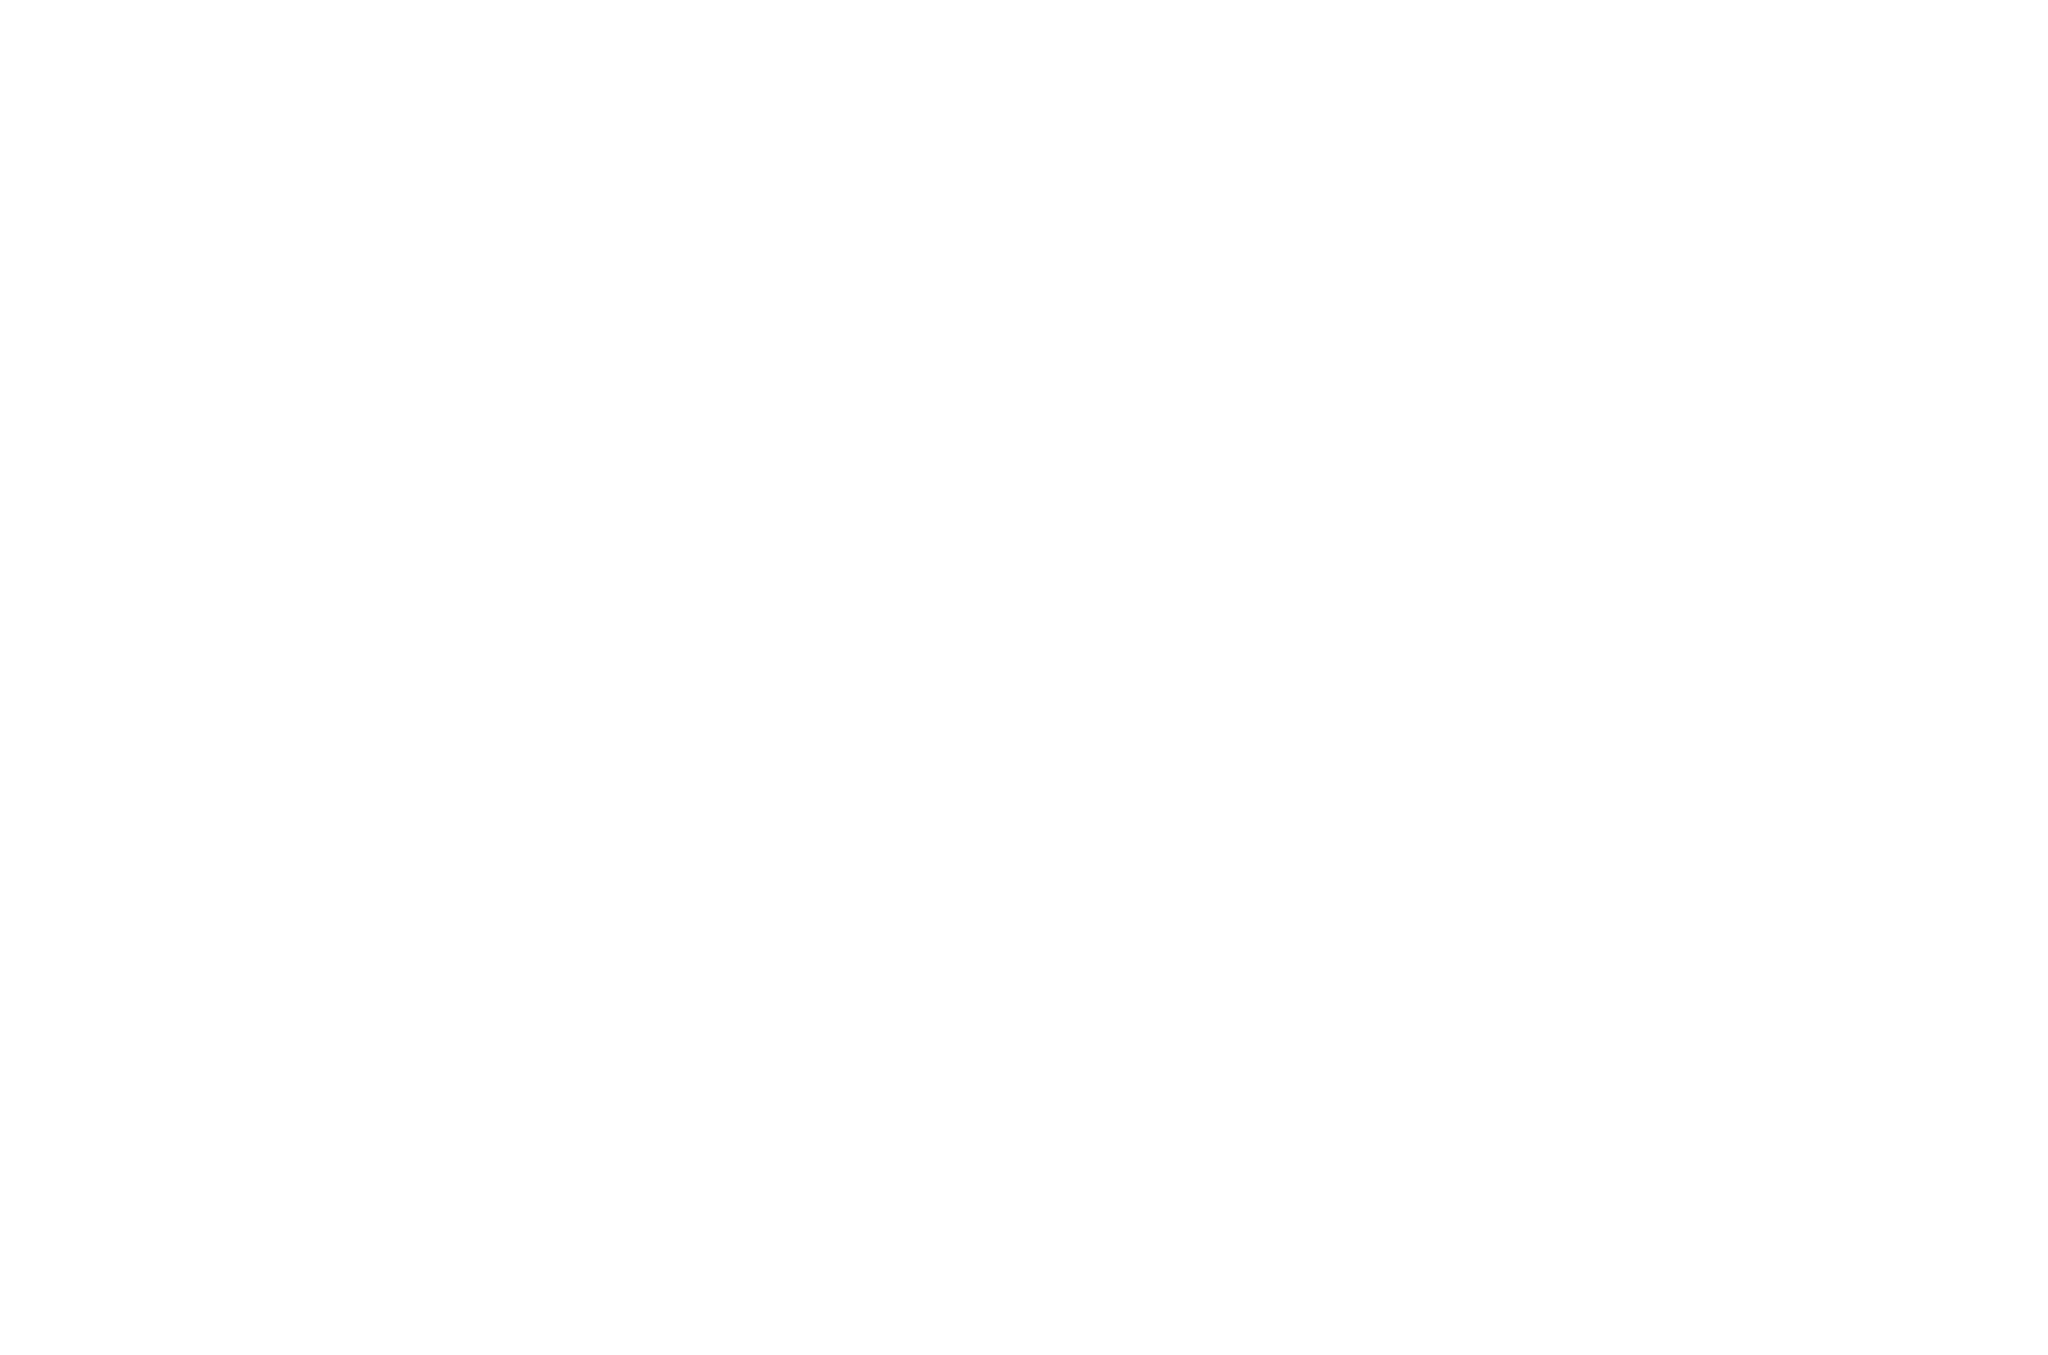
\includegraphics[width=\linewidth]{syscall-redirection.pdf}
\footnotesize
\caption{System call redirection for \thelibos{}.
In the normal case (the first instruction of \funcname{main}), \funcname{malloc} internally invokes 
\syscall{mmap}, which is redirected to \funcname{syscalldb} in \thelibos{}.\thelibos{} then invokes a \hostapi{}, \palcall{VirtMemAlloc}, to allocate host memory. The second instruction of \funcname{main} invokes a direct \linuxapi{}, which is trapped by the host-level exception handler,
and returned to \funcname{IllegalInstrHandler} in \thelibos{}.}
\label{fig:libos:syscall-redirection}
\end{figure}


\graphene{} modifies four \glibc{} libraries:
%When using \graphene{}, an application must be deployed with the modified \libc{} libraries,
the runtime loader (\code{ld.so}), the core library (\code{libc.so}), the pthread library (\libpthread{}), and the dynamic loading library (\libdl{}).
Each of the \Glibc{} libraries has separate purposes and features,
and is mostly loaded on demand except \code{ld.so}.
%Despite that \glibc{} has partitioned its code into separate libraries,
\graphene{} only modifies the \glibc{} libraries which contains direct \assembly{syscall} instructions.
%not every libraries of \glibc{} need to be modified for \linuxapi{} redirection.
%Only \code{libc.so}, \libpthread{}, and \libdl{} have included \code{syscall} instructions,
%and thus have to be modified for \graphene{}.
Other libraries, such as \code{libm.so},
only rely on 
existing \libc{} functions,
so \graphene{} leaves these libraries unmodified.



\paragraph{Hard-coded \linuxapis{}.}
Static binaries, or some platform-dependent applications, contain hard-coded \assembly{syscall} instructions
which cannot be redirected by a modified \libc{}.
Application developers
create a static binary with with hard-coded \linuxapis{} by statically linking a local version of \libc{} as part of the binary.
%as a static binary with hard-coded \linuxapis{}. %\code{syscall} instructions.
It is also possible to program an application
with assembly code that directly invokes \linuxapis{}---usually in a language runtime (e.g., the go runtime) or a system software (e.g., \projname{busybox}).
%---with assembly code that directly invokes
%platform-depenedent,
%rare \linuxapis{} that are not wrapped by \libc{} functions.
%one of the \linuxapi{} wrappers in \libc{}, or \funcname{syscall}.
%As a result, a ELF binary may contain hard-coded \assembly{syscall} instructions.
%Either way leads to hard-coding \code{syscall} instructions in the ELF binaries.
Because a modified \libc{} cannot redirect hard-coded \linuxapis{},
the application switches context into the host kernel,
causing security and compatibility breaches by exposing unauthorized or unsynchronized host OS states to the application.



\thelibos{} needs support from a host OS to restrict direct \linuxapis{} from an application instead of \libc{}.
%\thelibos{} depends on host-level \linuxapi{} restriction to redirect hard-coded \linuxapis{}.
%to prevent \linuxapis{} from anywhere other than a PAL.
A Linux kernel allows an application to install a \linuxapi{} filter in the Berkeley Packet Filter (BPF) format,
called a SECCOMP filter~\cite{seccomp}.
A SECCOMP filter can block or forward a \linuxapi{} based on the \linuxapi{} number,
argument values, or the code address that invokes the \linuxapi{}.
%A direct \linuxapi{} traps into the host kernel,
%unless the host has virtualized the interrupt handler to the \libos{}.
\graphene{} relies on the hosts to install a \linuxapi{} filter, or enforce architectural restriction, to detect direct \linuxapis{}.
For example, SGX already has a restriction that an enclave application cannot trigger any \linuxapi{} to switch context into the untrusted kernel.
% inside an enclave and triggers an exception for an in-enclave \linuxapi{}.
%\code{syscall} instructions
%(e.g., SGX restriction).
%The details of the \linuxapi{} restriction mechanisms are discussed in
%\fixme{update labels}
%Section~\ref{sec:linux:syscall} and Section~\ref{sec:sgx:syscall}.
If the host detects a direct \linuxapi{} from an application,
it can return
a PAL exception to an exception handlers assigned by \thelibos{}, using  \palcall{ExceptionSetHandler}.
%\thehostabi{} specifies that the host captures unauthorizes \linuxapis{}
%and redirects to an exception handler (set up by \palcall{ExceptionSetHandler}).
%If a binary makes an illegal \linuxapi{},
%the host-level \linuxapi{} restriction will trigger an \code{ILLEGAL} exception
%at \thehostabi{},
%and thus the \linuxapi{} is redirected by an exception handler
%assigned by \thelibos{}.
The exception handler can recover the \linuxapi{} number and arguments
from the context saved at the \linuxapi{},
and forward the \linuxapi{} to the \linuxapi{} handler
inside \thelibos{}.


Using exceptions to forward direct \linuxapi{} is much slower than redirecting through a modified \libc{},
due to the overhead of switching context between the application and the host kernel.
To handle an exception from the host OS,
the application at least switches context twice, including both triggering the exception handler and returning to the original execution.
To mitigate the overhead,
\thelibos{} can 
rewrite the hard-coded \assembly{syscall} or \assembly{int \$80} inside each application binary during the run time.
% to redirect the hard-coded \linuxapis{};
%use {\bf binary translation} to modify the hard-coded \code{syscall} instructions;
There can be two timings for rewriting the instructions:
One is the timing when the runtime loader a new binary, and \thelibos{} can perform a full scan of the binary
to replace \assembly{syscall} or \assembly{int \$80} with a jump to \thelibos{}'s \linuxapi{} table.
\thelibos{} can also passively replace the instructions
whenever the host detects a direct \linuxapi{} and triggers an exception handler.
%binary translation
%can be triggered when a host-level exception is raised
%for an illegal \linuxapi{},
%to optimize consecutive \linuxapi{} invocation at the same location.
%\thelibos{} can also perform a full scan in application binaries
%to spot and modify hard-code \code{syscall} instructions.
\graphene{} leaves binary rewriting
as a future feature.



%\papersection{Automatic Partitioning of JAVA Applications}
\label{sec:partitioning}
\sysname{} reduces the TCB of a security critical 
application by automatically partitioning the 
application into trusted and untrusted parts. It is not 
easy for a novice developer to find the right 
partitioning boundary. As a result, the developer may 
include classes, which are not necessary for operation, 
in the trusted part. These extra classes may expose new 
attack vectors, reducing the security of the enclave. 
\sysname{} provides an enclave image utility to help 
the developer partition the code with minimum effort. 
The developer only needs to identify the classes that 
represent the secure objects.

The enclave image utility calculates the transitive 
closure of dependencies of the secure object classes.
The tool traverses all the imported classes by secure 
classes and marks them as secure too. The tool keeps 
traversing the newly added secure classes until there 
is no new class to be marked secure. It not only 
follows the user-defined classes but also the system 
classes to create a list of all the secure classes.

The utility then replaces the references of secure classes in the untrusted part with proxy stubs to make a remote method call instead of direct method invocation. The tool uses Phosphor information  flow tracking library to instrument the secure classes so that the information flow can be tracked at runtime as explained in Section ~\ref{sec:info-leak}. The output of the tool is an instrumented secure classes JAR and another JAR containing untrusted code with proxy stubs.

The enclave image tool then packages the Graphene LibOS, JVM, JNI, and the instrumented trusted JAR together, and generates the enclave object by cryptographically signing the package using its private key and \fixmebj{XX} algorithm. The untrusted JAR and the enclave object are deployed together in the cloud machine with \sgx{} capability. 

Thus, the automatic partition tool reduces the attack vectors exposed in the enclave, and removes the burden of the developer to create the partition boundary by finding the entry/exit points. This enforces a strict smallest possible TCB for the secure application.

%%\section{Minimizing the TCB with the Non-Partitioned Model}

%\subsection{Reducing the TCB in \libos{}}
%\subsection{Partitioning the TCB in Multi-Process Applications}



%\section{Seamless Provisioning of Secure Objects and Classes}
\label{sec:provisioning}

%\section{Implementation Details}
\label{sec:civet:impl}

In this section, we discuss in detail about how the framework of \sysname{}
is implemented. 


\paragraph{Graphene library OS for \sgx{}.}
Similar to Drawbridge in Haven, Graphene \libos{} can map a larger number of system interfaces
to a much narrower host interface.
The untrusted interface of Graphene libOS after porting to \sgx{}
is mostly identical to the original host interface,
therefore Graphene libOS has a finite  bound on interface for the enclave.

Graphene libOS uses checksums of files to verify the integrity of supporting binaries and configuration.
The checksums of files are collected by a compile-time Signer tool of Graphene libOS.
The Signer tool ensures the integrity of the file checksums
by including them as part of the enclave's measurement.
Even if the same Graphene libOS is used
to run the applications,
different binaries in the enclaves yield different measurements. 
Such a design decouples the problem of distributing the library OS
and guaranteeing code integrity for each application, as the enclave integrity is based on the integrity of the application --- not just the \libos{}.
 
\sysname{} makes minor modifications to Graphene \libos{} to allow
the enclave to run
in the same process as the the untrusted \java{} VM.
The trusted and untrusted VM share a ring buffer (as shown in ~\ref{fig:civet:runtime} for communication during control transfer,
but the ring buffer itself is not trusted. The \sysname{} framework encrypts tainted security-sensitive data before passing the data on the ring buffer.
 
\paragraph{Control transfer at enclave entry.}

\sysname{} transparently transfers the control from the untrusted classes to trusted classes --- triggering enclave entry in the process ---
by intercepting the trusted classes's method or constructor invocation by untrusted classes.
\sysname{} intercepts in 2 cases:
(a) For an entry class that has finite entry points,
\sysname{} creates a bogus class that redirects all the constructors and static methods to the enclave.
(b) For other trusted classes, the \sysname{} adds the redirection calls only when a reference is returned by the enclave.
%(b) For other trusted classes, the interception is installed when a reference of 
%object is returned to the untrusted classes.
On future access of the object in the enclave, a proxy object is created to trigger the interception, using CGLib.

When the control transfers between the trusted and untrusted classes,
the arguments and return values of the methods
are stored in the ring buffer.
\sysname{} relies on serialization and deserialization to safely transfer object in and out of the enclave.
When \sysname{} deserializes an object, the \java{} VM perform type-checking on the object to sanity check the members.

After \sysname{} transfers the arguments, the \java{} VM thread that
invoke the intercepted  method does not directly enter the enclave.
On the other hand, several enclave threads that are pre-created during the enclave creation that are block-waiting on the ring buffer.
One of the enclave threads consumes the queued job, invokes the method,
and returns to block-waiting for more new requests.
No variable on the stack has to be persistent for the enclave threads,
and only instances of the trusted classes are persisted across enclave entry and exit.

Moreover, upon enclave entry and exit, the objects that can be safely transferred in or out of the enclave must be serialized / deserialized.
However, not all classes implement the interface {\tt Serializable},
especially when the classes contain internal states that cannot be simply interpreted.
But, \sysname{} assumes that the types of all arguments and return objects must be {\tt Serializable}. 

\paragraph{Framework limitations.}

As we leverage dependency tracking for automated partition, there are few corner cases that the Shredder cannot gracefully handle.
Because CGLib creates subclasses of objects when intercepting them,
it requires the intercepted object to be never finalized.
If a trusted class is also a final class, developers have to manually modify the class definition. Even though final attribute prevents further extension of the class, we argue that the application developer who is building the enclave can safely remove the final attribute as the \sysname{} signs the enclave jar.

 We also do not let trusted classes make method or constructor invocation of the untrusted classes, as the untrusted classes may be able to influence and interfere with the execution of trusted classes. Moreover, we only consider the provisioned code and data as security-sensitive. Even though this limits the usage scenarios, we argue that for any right usage of \sgx{} hardware, these limitations are not disruptive.

\section{Implementation Details}
\label{sec:implementation}

In this section, we discuss in detail about how the framework of \sysname{}
is implemented. 

\paragraph{The \graphene{} \libos{} ported to \sgx{}}
Similar to Drawbridge~\cite{porter11drawbridge}
in Haven~\cite{baumann14haven},
\graphene{}~\cite{tsai14graphene} maps a larger number of Linux system APIs
to a narrow, portable host interface.
Library OSes like Drawbridge and Haven unlock the platform limitations of \sgx{} and
allows many applications to be ported to enclave painlessly.
%The untrusted interface of \graphene{} \libos{} after porting to \sgx{}
%is mostly identical to the original host interface,
%therefore \graphene{} has a finite  bound on interface for the enclave.

%\graphene{} uses checksums to verify the integrity of applications.
%The checksums are collected by a compile-time Signer tool of \graphene{}.
%The Signer tool ensures the integrity of the file checksums
%by including them as part of the enclave's measurement.
%Even if the same \libos{} is used
%to run the applications,
%different binaries in the enclaves yield different measurements. 
%Such a design decouples the problem of distributing 
%and guaranteeing code integrity for each application, as the enclave integrity is based on the integrity of the application --- not just the libOS.
 
\sysname{} makes minor modifications to \graphene{} to allow
the enclave to run
in the same process as the the untrusted \jvm{}.
The trusted and untrusted VM share a ring buffer (as shown in Figure~\ref{fig:runtime} for communication during control transfer,
but the ring buffer itself is not trusted. The \sysname{} framework encrypts tainted security-sensitive data before passing the data on the ring buffer.
 
\paragraph{Control transfer at enclave entry}

\sysname{} transparently transfers the control from the untrusted classes to trusted classes --- triggering enclave entry in the process ---
by intercepting the trusted classes's method or constructor invocation by untrusted classes.
\sysname{} intercepts classes in two ways:
(a) For an entry class that has finite entry points,
\sysname{} creates a wrapper class that redirects all constructors and static methods.
(b) For other trusted classes, \sysname{} adds the redirection calls only when a reference is returned by the enclave. %\fixmebj{Is this correct?}
%(b) For other trusted classes, the interception is installed when a reference of 
%object is returned to the untrusted classes.
On future access of the object in the enclave, a proxy object is created to trigger the interception, using CGLib.

When the control transfers between the trusted and untrusted classes,
the arguments and return values of the methods
are stored in the ring buffer.
\sysname{} relies on serialization and deserialization to safely transfer object in and out of the enclave.
When \sysname{} deserializes an object, the \jvm{} perform type-checking sanitize the input. % the members.

%After \sysname{} transfers the arguments, the \jvm{} thread that
%invoke the intercepted  method does not directly enter the enclave.
%On the other hand, several enclave threads that are pre-created during the enclave creation that are block-waiting on the ring buffer.
%One of the enclave threads consumes the queued job, invokes the method,
%and returns to block-waiting for more new requests.
%No variable on the stack has to be persistent for the enclave threads,
%and only instances of the trusted classes are persisted across enclave entry and exit.

%Moreover, upon enclave entry and exit, the objects that can be safely transferred in or out of the enclave must be serialized / deserialized.
%However, not all classes implement the interface {\tt Serializable},
%especially when the classes contain internal states that cannot be simply interpreted.
%But, \sysname{} assumes that the types of all arguments and return objects must be {\tt Serializable}. 

\paragraph{Limitations}
As we leverage dependency tracking for automated partition, there are few corner cases that the Shredder cannot gracefully handle.
Because CGLib creates subclasses of objects when intercepting them,
it requires the intercepted object to be never finalized.
If a trusted class is also a final class, developers have to manually modify the class definition. Even though final attribute prevents further extension of the class, we argue that the application developer who is building the enclave can safely remove the final attribute as the \sysname{} signs the enclave jar.

 We also do not let trusted classes make method or constructor invocation of the untrusted classes, as the untrusted classes may be able to influence and interfere with the execution of trusted classes. Moreover, we only consider the provisioned code and data as security-sensitive. Even though this limits the usage scenarios, we argue that for any right usage of \sgx{} hardware, these limitations are not disruptive.

%\input{Implementation Details}
%% ASPLOS
%\input{cloud}
%\input{Case Studies}
\papersection{Case Studies}
\label{sec:case-study}

%\fixmets{1 page} 
In order to evaluate the utility of \sysname{}, we partitioned
several example \java{} applications, which we use in our evaluation.


\paragraph{Session Encryption in SSH Client/Server}
%Code that handles security sensitive data
In order to show the ability of \sysname{} to protect 
confidential data and avoid leaking that data,
%A \java{} program with a secret that is either generated during runtime
%or provisioned from trusted remote enclaves,
%can be partitioned and secured by \sysname{} to prevent leaking the secret.
%We demonstrate this use case
%using 
we partitioned a \java{}-based SSH client and server~\cite{apache-sshd}.
In this case, the protected secret is the session key.
%For an SSH connection, one primary secret that needs to be secured
%is the session key used for encrypting and decrypting the data
%between the two communicating parties.
For both the SSH client and server, we create
a control class iDMn the enclave that includes 
the key generator, encryption engine objects, secret key
and the {\em BouncyCastle}~\cite{bouncycastle} cryptography library.
The rest of the application is outside of the enclave.
%from the rest of the application.
%\fixmedp{surprising the private key isn't also in the enclave}

We use information flow tracking to ensure that the only data
leaving the enclave is ciphertext output from the encryption algorithm,
or plaintext returned from the decryption algorithm.
%This involves adding lines to the end of both algorithms, and does assume that
%the encryption and decryption functions are implemented correctly.
Attempts to copy the session key directly into an output buffer at any other point in the code
will result in encryption of the buffer before leaving the enclave.

{\tt org.apache.sshd.common.SecurityUtils} is identified as the entry class for Shredder, because this class returns all the objects required for the SSH Protocol.
Shredder generates the enclave image that includes the secret key classes, random generator, key generator, engine for diffie-hellman key-exchange, and encryption-decryption engine. Both the client as well as the server are partitioned to be run using \sysname{}. The client and server first mutually attest each other, exchange the session key, and then setup the connection session.

%We use these SSH client and server for transferring files using SFTP. For simplicity, we run both client and the server on the same host, but in different enclaves. 
%We measure the bandwidth of file transfer as discussed in \S\ref{sec:eval:perf}

%\fixmedp{I took some liberty here: We have to be able to receive data too, right?  Also, I would be more careful with the use of ``guarantee'' in general}

%% The information flow filtering guarantees that no part of the session key
%% can leak from the enclave despite any vulnerabilities 
%% in the crypto library or the control class.
%% The only data that can be released from the enclave
%% is the cipher text of the inputs from the SSH client and server,
%% encrypted with the session key, after declassification.
%% We only had to add only one line of code to declassify the cipher text using the {\tt Enclave.declassify(ciphertext)} API. Thus, in addition to only identifying classes with sensitive information, the developers have to just add one statement per declassifying location in the enclave classes.

\paragraph{Secret Hadoop Algorithm}
%Code that contains a secret algorithm
\sysname{} not only protects confidential data, but also protects confidential code.
For instance, if a company has developed an analysis tool that gives them a essential competitive advantage,
they must either run their own data center or trust a cloud provider not to leak their tool 
to any competitors.
%, such 
%as trade secret, that developers intend to protect from insecure system stack.

To demonstrate this use case, we modify a Hadoop sort algorithm~\cite{hadoop-sort},
so that the implementation of its Partitioner, Mapper, Combiner, Sorter and Reducer
are isolated from the rest of the Hadoop infrastructure. 
The algorithm sorts values from a key-value store, in which
the input keys and values are encrypted.
The output of the sorting algorithm is a sorted, encrypted key value store.
%based on original values a key-value store, in which
%both input keys and values are encrypted.

The Hadoop framework schedules proxy Partitioners, Mappers, Combiners, Sorters, and Reducers,
and then creates enclaves for these classes.
Once a baseline \sysname{} enclave is created, encrypted class files
are downloaded from a trusted server using our remote attestation tools,
and then decrypted, loaded, and measured for integrity. 
%We evaluate the Job completion time for our sort algorithm in \S\ref{sec:eval:perf}.
%, requests for the real classes to be provisioned from a trusted server, loads, and executes the provisioned classes.

The information flow control at the enclave border protects against
accidental output of a plaintext key-value pair from the encrypted store,
as well as protects the class code file itself.
Similarly, intermediate state from the code cannot be inadvertently returned by a function to the untrusted Hadoop framework,
although we do allow encrypted outputs to be passed from a Mapper to a Combiner or Reducer.
The contents of any code cannot be leaked outside enclave by copying the code into an output object, as the tainted object is automatically encrypted before leaving enclave. %\fixmedp{does this just happen naturally?},
Also, in conjunction with the trusted remote server, we rate-limit instantiations of the code to mitigate the risk of
brute-force mapping of its outputs or reverse-engineering the code.

\begin{comment}
%% any output of the isolated classes ---
%% even if it is just an intermediate state ---
%% is encrypted before leaving the enclave.
%% \sysname{} not only protects the implementation of the algorithm,
%% but any output of the algorithm that may potentially help attackers
%% reverse-engineer the implementation. The {\em confidential code} property of ~\sysname{} is not limited to Hadoop, but can also be leveraged by standard \java{} applications.

\paragraph{Secure Data Manager Web-app.}
%JAVA Web-start Application
\sysname{} can also secure {\em Java Network Launch Protocol} (JNLP) applets and web-start apps, effectively 
extending trust from a remote trusted server to a client enclave using any web-app 
plugged into a supported browser. This allows the developers to offload some of the 
computation on secret data to the client machine from the trusted server.
%\java{} applications in the form of
%can also be secured by \sysname{}. 

For instance, in a large medical hospital with a centralized repository of patient data,
the doctors may want to access any patient data from any terminal using a web browser.
A web developer can design an applet such as Secure Data 
Manager(SDM)~\cite{sdm-applet} to store the secret patient data on a client machine, 
and display this information securely using Intel Protected Audio and Video Path 
(PAVP) technology~\cite{intel-pavp}.
However, to protect the sensitive patient information from untrusted system stack, the 
developer can use \sysname{} to isolate the classes that represent the secure data 
in an enclave. The developer just has to identify such classes representing the secret 
data and display methods, and the \sysname{} seamlessly creates enclave for 
managing secret data.
% or perform computations on secret data isolated in an enclave.
%We demonstrate this use case using a 
%\fixmedp{what is the practial use case?  Like, what is the data actually used for?}
The trusted data manager class authenticates the doctor and loads the provisioned data 
from the remote trusted server. The Intel PAVP enabled displays can then take the input from the display methods of the trusted data manager class.

For simplicity, we only partition and run the SDM applet from a browser without the support for Intel PAVP display devices. We identify four classes --- {\tt SafetyBox}, 
{\tt AuthenticationInfo}, {\tt LoginEntry}, and {\tt Type} --- as entry class to the Shredder and generate a web-start app image containing the enclave image. The web-app loads normally, and when it tries to access any of the above four classes, \sysname{} seamlessly creates an enclave for those objects. 
%We measure the latency of I/O from the SDM in \S\ref{sec:eval:perf}.


%\fixmedp{This last example is pretty content free.  Can you give me an example of a web app that would use this, and flesh out the story a bit?}
\end{comment}

\declarecommand{\sysname}{\graphene{}}
\declarecommand{\pal}{PAL}
\declarecommand{\syscalls}{131}
\declarecommand{\palcalls}{43}
\declarecommand{\nativecalls}{50}
\declarecommand{\gipclines}{1,131}
\declarecommand{\sandboxmodlines}{888}
\declarecommand{\reflines}{3,568}
\declarecommand{\libclines}{606}
\declarecommand{\interfacenum}{41}
\declarecommand{\light}{lighttpd}
\declarecommand{\gcc}{gcc}
\declarecommand{\lmbench}{LMbench}
\declarecommand{\ab}{ApacheBench}
\declarecommand{\busy}{Bash}
\declarecommand{\skylake}{Skylake}

\chapter{Evaluation}
\label{chap:eval}
%\chapter{Related Works}
\label{chap:related}

\makeatletter
\def\input@path{{related/}}
\makeatother
\graphicspath{{related/figures/}}

This chapter describes the formal definition of the \graphene{} host ABI.

\section{Basic Definitions}

The \graphene{} host ABI defines a set of {\em functions}, similar to the API of UNIX or POSIX.
The functions are directly called by the library OS, along with the arguments given either in the registers or on the stack.
A host-specific \graphene{} loader is responsible for resolving the linking, from the library OS to the host ABI.
\section{Library OSes and virtualization}





\paragraph{Previous library OSes.}
Previous library OSes~\citep{porter11drawbridge,xax,unikernels,baumann13bascule,osv}
focus on running single-process applications
in a \picoproc{} or a unikernel
for verious reasons including compatibility and security isolation.
%to support coordination abstractions required 
%for multi-process applications, such as shell scripts.
Bascule~\citep{baumann13bascule} implements a Linux library OS on a variant of the Drawbridge ABI,
but does not include support for multi-process abstractions such as signals or copy-on-write fork.
The Bascule Linux library OS also implements fewer Linux system calls than Graphene, missing
features such as signals.
Bascule demonstrates a complementary facility to Graphene's multi-process support: composable library OS extensions, 
such as speculation and record/replay.
OSv is a recent open-source, % project to design and implement a 
single-process 
library OS to support a managed language runtime, such as Java, on a bare-metal hypervisor~\citep{osv}.


A number of recent projects have provided a minimal, isolated environment
for web applications to download and execute native code~\citep{nacl,xax,howell13refactoring,gazelle,atlantis}.
The term ``picoprocess'' is adopted from some of these designs, and they share 
the goal of pushing system complexity out of the kernel and into the application.
%%% Despite these common design themes, the motivations
%%% for these projects varies widely, including
%%% robustly enforcing browser policy\citep{gazelle};
%%% ensuring that a web page is compatible with the JavaScript, CSS, and other interpreters in the browser~\citep{atlantis};
%%% and simply the ability to push code from the data center onto the client where it makes 
%%% sense~\citep{nacl, embassies, howell13refactoring}.
Unlike a library OS, these systems
generally sacrifice the ability to execute unmodified application code, 
eliminate common UNIX multi-process functionality (e.g., fork), or both.


The term library OS also refers to an older generation of research
focused on tailoring hardware management heuristics 
to individual application needs~\citep{kaashoek97exokernel,anderson92libos,cheriton94cache,leslie96nemesis,libra},
whereas newer library OSes, including Graphene, focus
on providing application compatibility
across different hosts without dragging along an entire legacy OS.
A common thread among all libOSes is moving functionality from the kernel
into applications and reducing the TCB size or attack surface.
Kaashoek et al.~\citep{kaashoek97exokernel} identify multi-processing as a problem for an Exokernel libOS,
and implemented some shared OS abstractions.
The Exokernel's sharing designs rely on shared memory rather than byte streams,
and would not work on recent libOSes,
nor will they facilitate dynamically sandboxing two processes.

%% In moving services out of the kernel and into user libraries our design resembles a microkernel~\citep{liedtke95sosp, Baron:1985:MOE}.
%% %liedtke93sosp,liedtke95sosp, Baron:1985:MOE, Jones:1986:MMK, Rashid:1987:RAM}.
%% An important distinction is that
%% microkernels generally centralize system services in a single trusted daemon,
%% whereas Graphene distributes management of coordination APIs among
%% cooperating guests.

\begin{comment}
Dune~\citep{belay12dune} %merges the concept of a process and VM,
leverages virtualization hardware 
to allow an application
to safely manage privileged CPU features
such as page tables and interrupts.
%Dune leverages virtualization hardware  to safely 
%isolate privileged hardware access within a process.
Dune's goals are complimentary to ours; we expect that
certain aspects of the PAL implementation would be simplified on Dune.
\end{comment}

User Mode Linux~\citep{user-mode-linux} (UML) executes a Linux kernel inside a process
by replacing  architecture-specific code with 
code 
that uses Linux host system calls. % to emulate this functionality.
%Because UML runs a complete Linux kernel and multiple processes,
%it is effectively
UML is best described as  an alternative approach to paravirtualization~\citep{barham03xen},
and, unlike a library OS, does not deduplicate functionality.


\paragraph{Virtualization.}
Recent library OSes, including Graphene,
search for a better
division of labor between the host kernel and guests.
Paravirtualized VMs attempt to move away from modeling specific hardware designs in software
toward a more virtualization-friendly hardware model~\citep{barham03xen,whitaker02denali, eiraku09outsourcing}.
Library OSes can be viewed as extreme paravirtualization---attempting
to find the most ideal interface between guest and host. %abstractions of hardware without also baking-in host semantics.



\paragraph{Distributed coordination.}
Distributed operating systems,such as LOCUS~\citep{locus83sosp,fleisch86locus}, Amoeba~\citep{mullender90amoeba,cheriton89naming} and  
Athena~\citep{champine90athena} required a consistent namespace for process identifiers and other IPC abstractions
across physical machines.
%A key requirement for naming in a distributed OS is network transparency---that the name should be independent of the physical placement of an object in the system.
Like microkernels, these systems generally centralize all management in a single, system-wide service.
%For instance, Amoeba has a single session server that allocates process identifiers.
%This system service may be replicated or partitioned for improved performance on a large network or to
%divide management responsibility across administrative domains~\citep{cheriton89naming}.
%Each Graphene guest also needs to coordinate naming of Unix abstractions, such as processes or System V IPC keys.
%Although Graphene draws some inspiration from these distributed OSes, 
%Graphene's goals and usage model are different, and 
Rote adoption of a central name service does not meet our goals
of security isolation and host independence.

Several aspects of the Graphene host kernel ABI are similar to the
Plan 9 design~\citep{pike90plan9}, including the unioned view of the host file system
and the inter-picoprocess byte stream.
Plan 9 demonstrates how to implement this host kernel ABI,
whereas Graphene uses a similar ABI 
to encapsulate multi-process coordination 
in the libOS.

%% or coordinating coordinate a distributed file system
%% across multiple workstations,
%% but rather to demonstrate how it can be leveraged to 
%% implement a more efficient guest library OS. instance, Plan 9 uses the 9P protocol to coordinate a distributed file system
%% across multiple workstations. In contrast, Graphene uses streams




Barrelfish~\citep{baumann09barrelfish} argues that multi-core scaling is best served 
by replicating shared kernel abstractions at every core, and using message passing 
to coordinate updates at each replica, as opposed to using cache coherence to update a shared data structure.  
Barrelfish is a new OS; in contrast,
Cerberus~\citep{song11eurosys} applies similar ideas to coordinate abstractions
across multiple Linux VMs running on Xen.
%Cerberus coordinates a unified view of the process tree, file system, network card,
%and the address space when threads run on separate cores---forwarding 
%some system calls to other kernels as remote procedure calls.
In order for a library OS to provide multi-process abstractions, 
Graphene must solve some similar problems, but innovates by
replicating additional classes of coordination abstractions, such as System V IPC,
and facilitates dynamic sandboxing.
%and optimizes performance through 
%techniques such as lazy discovery.
The focus of this paper is not on multi-core scalability, but on security isolation and compatibility with legacy, multi-process applications.
That said, we expect that systems like Barrelfish~\citep{baumann09barrelfish} 
could leverage our implementation techniques to efficiently 
construct higher-level OS abstractions, such as System V IPC and signals.

%% We note that several recent projects argue that multi-core scalability 
%% is enhanced by eschewing cache coherence and shared data structures, 
%% in favor of a similar 
%% design which
%% replicates state across cores
%% {\em within an OS kernel}~\citep{baumann09barrelfish} or {\em across legacy guest OSes}~\citep{song11eurosys}.
%% The focus of this paper is not on multi-core scalability, but on security isolation and compatibility with legacy, multi-process applications.
%% That said, we expect that systems like Barrelfish~\citep{baumann09barrelfish} 
%% could leverage our implementation techniques to efficiently 
%% construct higher-level OS abstractions, such as System V IPC and signals.

L3 introduced a ``clans and chiefs'' model of IPC redirection, in which IPC to
a non-sibling process was validated by a the parent (``chief'') before a message could leave the clan~\citep{liedtke92clans}.
%This model was primarily used to enforce access control on system abstractions,
%and abandoned for capabilities on kernel objects in L4
Although this model was abandoned as cumbersome for general-purpose access control~\citep{elphinstone13microkernels},
the Graphene sandbox design observes
that a stricter variation is a natural fit
for security isolation among multi-process applications.

Cerberus focuses on replicating lower-level state, such as process address spaces
which Graphene leaves in the host kernel.
As a result, the performance characteristics are different.
Although this comparison is rough, 
we replicated their test of ping-ponging 1000 
{\tt SIGUSR1} signals and compare the ratio to their reported data, 
albeit with different hardware and our baseline kernel is newer 
(3.2 vs 2.6.18).  
When signals are sent inside of a single guest on Graphene, they are {\em faster}
by 79\%, whereas performance drops by a 5.5--18$\times$ on Cerberus.
When passing signals across coordinating guests both approaches are competitive:
Graphene's cross-process signal delivery is 4.6$\times$ slower than native, whereas Cerberus ranges from 
3.3--11.3$\times$ slower, depending on the hardware.


%% For instance, Graphene guests may require a mixture of isolated and shared namespaces.
%% Moreover, Graphene naming must support dynamic detachment of one guest from a confederation of other guests.
%% Our work contributes  an implementation of distributed naming inside the library OS, facilitating security isolation, 
%% and application-transparent detachment.

\paragraph{Migration and security isolation.}
Researchers have added checkpoint and migration support to Linux~\citep{linux-cr}
by serializing kernel data structures to a file
and reloading them later.  
This introduces several challenges, including
security concerns of loading data structures into the OS kernel from a potentially 
untrusted source.
%, as well as significant engineering and maintenance effort.
In contrast, Graphene checkpoint/restore 
%on a simple host ABI
requires little more than a guest memory dump.
%The host state can be easily restricted by a sandbox.

%% supports migration of one or more process across
%% hosts with the same kernel.
%% To maintain consistency of namespace and resource throughout migration,
%% Zap provides a thin virtualization layer upon which
%% application can have the same virtualized and conflict-free view of system.
%% To simplify process dependency that complicates migration, Zap migrates
%% processes in the unit of Pods, a container with virtualized namespace,
%% memory checkpoints and private file system. 

%Docker - http://www.docker.io/ - really looks like it just automates creation of a minimal hard drive

OS-based virtualization, such as 
Linux VServer~\citep{vserver},  containers~\citep{bhattiprolu08containers},
and Solaris Zones~\citep{price04zones},
implement security isolation by maintaining multiple copies of kernel data structures,
such as the process tree,
in the host kernel's address space.
In order to facilitate sandboxing, 
Linux has added support for launching single processes
with isolated views of namespaces, including process IDs and network interfaces~\citep{lwn-namespaces}.
FreeBSD jails apply a similar approach to augment an isolated {\tt chroot} environment
with other isolated namespaces, including the network and hostname~\citep{jails}.
Similarly, Zap~\citep{osman02zap} migrates groups of process, called a Pod,
which includes a thin layer virtualizing system resource names.
In these approaches, all guests must use the same OS API, and the host kernel
still exposes hundreds of system calls to all guests.
Library OSes move these data structures into the guest, enabling
a range of personalities to run on a single guest and limiting the attack surface
of the host.


Shuttle~\citep{shan12shuttle} permits selective violations of strict isolation
to communicate with host services 
under OS-based virtualization.
For example, collaborating applications may communicate using the Windows Common Object Model (COM);
Shuttle develops a model to permit access to the host COM service.
%Windows guest applications 
%may rely on the host's Service Control Manager
%for certain functionality, and this functionality cannot be replicated inside of each guest.
%Similarly, some collaborating applications may 
Rather than attempting to secure host services,
Graphene moves these services out of the host
and into collaborating guests.


%From an API perspective, this is similar to Graphene's isolation.  
%This approach requires all applications to run on the same host kernel,
%and 
%However, these approaches are implemented in the same address space 
%as the host kernel and still expose a wide attack surface area.  
%The library OS
%approach moves much of this attack surface area out of the kernel and into the guest.

\section{Graphene on SGX}
\label{sec:eval:sgx}

%This section will shows the evaluation results of the \graphenesgx{} framework,
%in term of performance, security, and compatibility to Linux.

%\subsection{Performance Evaluation}
\label{sec:eval:perf}


%We evaluate the performance overheads on running unmodified Linux applications
%on SGX.
%Unlike the existing \sgx{} shielding systems which focuses on cloud-based systems or microservices,
\graphenesgx{} is designed to be general-purpose, supporting a broad range of
server and command-line applications. 
%, including both server and desktop workloads.
%\fixmedp{I wouldn't really call gcc or R ``desktop''}
\fixme{get rid of the part that we need to compile source code}
We thus evaluate performance overheads of unmodified Linux applications, using binaries 
from an Ubuntu installation.
%, or,
%in the case of Apache, Lighttpd, and NGINX,
%compiled from original source code using the default configurations.}
%(Apache, Lighttpd, and NGINX are compiled from source).} %\fixmedp{which apps are compiled?}
Depending on the workload, we measure application throughput or latency.
%According to the types of workloads, we design experiments to evaluate whether \graphenesgx{} can support applications with acceptable throughput or latency.

%All applications in our experiments are real, unmodified Linux applications,
%either directly taken from a disk with Ubuntu installation,
%or compiled using the default configuration given by the developers.
%No source code modification or change of compilation environment is required in the experiments.
%In our experiments, we either test on application binaries taken off-the-shelf from the Ubuntu {\tt APT} repositories,
%or applications that are built from the default configurations
%provided by the developers.
%Either source code modification or adjustment of the compilation environment is avoided in the setup of experiments.
%Our evaluation simulates the realistic results of running unmodified Linux applications in \graphenesgx{}.
%running Linux COTS applications on commodity hardware.

In order to differentiate SGX-specific overheads 
from Graphene overheads,
%, which also
%runs on a Linux host without SGX, 
we use both
Linux processes and \graphene{} on a Linux host without SGX as baselines
for comparison.
%Since a large portion of the \libos{} design is inherited from the \graphene{} \libos{},
%the performance impact of adopting \graphenesgx{} is largely affected by the design choices made in \graphene{}.
%In order to show the performance impact of \graphenesgx{} over \graphene{}, we use both native Linux and \graphene{} on a Linux host as the baselines for comparison.
Note that \graphene{} includes two optional kernel extensions:
one that creates a reference monitor to protect the host kernel from 
the library OS, and one that optimizes fork by 
with copy-on-write for large (page-sized) RPC messages.
%implementing a multi-page RPC
%abstraction.
Neither of these extensions are currently supported in \graphenesgx{}.
%so we measure baseline Graphene with these disabled.
% can be optionally run with a reference monitor for security isolation, and a bulk IPC abstraction for fork optimization.
%Since neither of the features is ported in \graphenesgx{},
%we mostly compare \graphenesgx{} to \graphene{} with these two features disabled,
%to show a more meaningful comparison.

% Put figures at the front
\begin{figure*}[t!]
\centering

\begin{minipage}{.3\textwidth}
\centering
\footnotesize
\includegraphics[width=\linewidth]{sgx/lighttpd-throughput-latency}\\
{\bf (a) Lighttpd (25 threads)}
\end{minipage}
\begin{minipage}{.3\textwidth}
\centering
\footnotesize
\includegraphics[width=\linewidth]{sgx/apache-throughput-latency}\\
{\bf (b) Apache (5 processes)}
\end{minipage}
\begin{minipage}{.3\textwidth}
\centering
\footnotesize
\includegraphics[width=\linewidth]{sgx/nginx-throughput-latency}\\
{\bf (c) NGINX (event-driven)}
\end{minipage}

\caption{Throughput versus latency of web server workloads, including Lighttpd, Apache, and NGINX, on native Linux, \graphene{}, and \graphenesgx{}.
We use an ApacheBench client to gradually increase load, and plot
throughput versus latency at each point.  Lower and further right
is better.
%\fixmedp{RB: Add another sentence or two to explain what the experiment is and how to interpret} }
}
\label{fig:server-throughput-latency}
\end{figure*}


\fixmedp{RA asks for a limitations section; I don't think we should do this, but the expensive stuff (events, fork, open) we should add as much as we can about what, if anything,  can be done about it, and what can't without more hardware}

\paragraph{Experimental setup.}

We use a Dell Optiplex 790 Small-Form Desktop,
with a 4-core 3.20 GHz Intel Core i5-6500 CPU (no hyper-threading, with 6MB cache),
8 GB RAM, and a 512GB, 7200 RPM SATA disk.
%We disable SpeedStep and TurboBoost to prevent interference.
The host OS is Ubuntu 16.04.4 LTS, with Linux kernel 4.4.0-21.
Each machine uses a 1Gbps Ethernet card connected to a dedicated local network.
We use version 1.8 of 
the Intel \sgx{} Linux SDK~\cite{intel-sgx-linux-sdk} and driver~\cite{intel-sgx-linux-driver}.
%We measure version 0.4beta of \graphene{}.

%Adding more detail of KVM environment
%Unless otherwise noted, \graphenesgx{} measurements include the Phosphor instrumentation.

\subsection{Server applications}

One deployment model for SGX is to host network services
on an untrusted cloud provider's hardware.
%To measure this case, 
We measure three widely-used Linux web servers, including {\bf Lighttpd}~\cite{lighttpd} (v1.4.35), {\bf Apache}~\cite{apache} (v2.4.18), and {\bf NGINX}~\cite{nginx} (v1.10).
%, to evaluate the performance of server-type workloads in \graphenesgx{}.
%These applications are all sophisticated, non-trivial workloads, and are constantly being used for commercial purposes.
%We test these applications to evaluating significantly different execution patterns, to benchmark the performance of \graphenesgx{} under each circumstances.
%Also, we do not explicitly configure these servers to secure their payloads using the HTTPS protocol.\fixme{if have time, maybe try again with HTTPS}
For each workload, we use ApacheBench~\cite{apachebench} to download the web pages on a separate machine.
%\edit{over Gigabit LAN}. %\fixmedp{more specific?}
%across a high-speed \fixmedp{Can you say
%more specifically the specs, like 10 GBps or whatever; also, if this is the same vlan, I might just describe this as being on a LAN, minimizing interference} University network.
The concurrency of ApacheBench is gradually increased during the experiment, to test the both the per-request latency and the overall throughput of the server.
Figure~\ref{fig:server-throughput-latency} shows the throughput versus latency of these server applications
in \graphenesgx{}, \graphene{} and Linux. 
Each workload is discussed below.

{\bf Lighttpd}~\cite{lighttpd} is a web server designed to be light-weight, yet robust enough for commercial uses. 
Lighttpd is multi-threaded; we test with 25 threads to process HTTP requests. 
By default, Lighttpd uses the \syscall{epoll\_wait} system call to poll listening sockets.
At peak throughput and load,  both \graphene{} and \graphenesgx{} have marginal overhead on either latency or throughput of the Lighttpd server.
The overheads of \graphene{} are more apparent when the system
is more lightly loaded, at 
%When Lighttpd is not overloaded, \graphenesgx{} causes 
15--35\% higher response time, or 13--26\% lower throughput. 
Without SGX, \graphene{} induces 
11--15\% higher latency or 13-17\% lower throughput over Linux;
the remaining overheads are attributable to SGX---either hardware or our OS shield.
%platform adaptation layer (PAL) code.

%\fixmedp{Some more detailed analysis would be nice.}
%Only part of this overhead is contributed by the library OS implementation, since using \graphene{} without \sgx{} causes only 

%\fixmedp{Why did you comment this out?  Let's discuss: Does it really make sense to have two points at the same  x-axis value?  Perhaps the axes should be inverted?  I'm not really sure about the methodology, but something about the line doubling back on itself seems wrong.  Maybe you want to separate these and show throughput vs. load, and a CDF of latencies?}


{\bf Apache}~\cite{apache} is one of the most popular production web servers. We test Apache using 5 preforked worker processes to service HTTP requests,
in order to 
to evaluate the efficiency of \graphenesgx{} across enclaves.
%n server, 
%In the experiment, the Apache server creates 5 preforked processes which coordinate on processing HTTP requests.
This application uses IPC extensively---the preforked processes of a server use a System V semaphore to synchronize on each connection.
%When receiving a connection, the preforked processes of Apache will coordinate among themselves using the system V IPC semaphores.
Regardless of the workload, the response time on \graphenesgx{} is 12--35\% higher than Linux, due to the overhead of coordination across enclaves over encrypted RPC streams.
The peak throughput achieved by Apache running in \graphenesgx{} is 26\% lower than running in Linux.
In this workload, most of the overheads are SGX-specific, such as exiting enclaves when accessing the RPC, as non-SGX Graphene
has only 2--8\% overhead compared to Linux.

%The enclave restriction \fixmedp{Huh?} is the main contributor to this overhead, as \graphene{} generally only causes 2--8\% overhead.

%\fixmedp{Check the lightttp graph; the lines are right on top of each other, and dont' look 22\% apart to me.  Some of this may be the scale of the y axis}

{\bf NGINX}~\cite{nginx} is a relatively new web server designed for high programmability, for as a building block to implement different services.
Unlike the other two web servers, NGINX is event-driven and mostly configured as single-threaded.
%When running as a simple HTTP server, NGINX uses an event-driven model instead of multi-threading/multi-processing to handle incoming requests.
\graphenesgx{} currently only supports synchronous I/O at the enclave boundary,
and so, under load, it cannot as effectively overlap I/O and computation
as other systems that have batched and asynchronous system calls.
%Asynchronous system calls and events in general are less mature features of
%\graphenesgx{}, and, 
Once sufficiently loaded, NGINX on both \graphene{} and \graphenesgx{} 
performs worse than in a  Linux process. % once sufficiently loaded.
%We observe that both \graphene{} and \graphenesgx{} tend to perform poorly in an event-driven server.
The peak throughput of \graphenesgx{} is 1.5$\times$ lower than Linux;
without SGX, Graphene only reaches 79\% of Linux's peak throughput.
%\fixmedp{Maybe shout out to eleos, or cite other work}
We expect that using tools like Eleos~\cite{orenbach17eleos} to reduce exits
would help this workload; in future work, we will improve
asynchronous I/O in \graphenesgx{}.

%\graphenesgx{} causes 17--90\% more response time when the server is not overloaded,
%but up to 1.5$\times$ at the peak throughput.
%If we compare the peak throughput with native Linux, \graphenesgx{} is 70\% less.
%\graphene{} also suffers the same performance pattern, as the throughput drops dramatically after reaching 79\% of the peak throughput of NGINX in Linux.
%The reason of the slowdown is that the host interface of \graphene{} and \graphenesgx{} only supports synchronous IO, so implementing asynchronous IO will be less efficient. This limitation is a trade-off to the portability of \graphene{}.
%\fixmedp{Didn't get the portability point; please spell out what you meant, if important}

\begin{figure*}[t!]
\centering

\begin{minipage}{.4\textwidth}
\centering
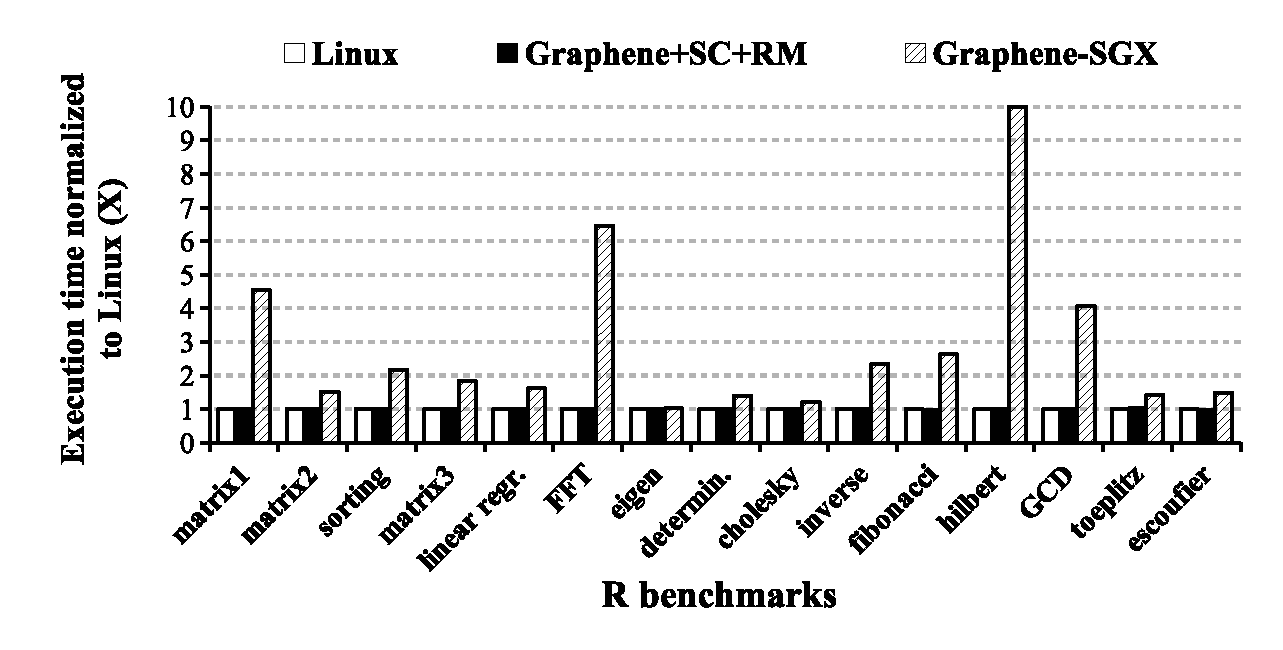
\includegraphics[width=\linewidth]{sgx/r-overhead}\\
{\bf (a) R}
\end{minipage}
\begin{minipage}{.275\textwidth}
\centering
\includegraphics[width=\linewidth]{sgx/gcc-overhead}\\
{\bf (b) GCC}
\end{minipage}
\begin{minipage}{.25\textwidth}
\centering
\includegraphics[width=\linewidth]{sgx/curl-overhead}\\
{\bf (c) CURL}
\end{minipage}

\caption{Performance overhead on desktop applications, including latency of R, execution time of GCC compilation, download time with CURL. The evaluation compares native Linux, \graphene{}, and \graphenesgx{}.} %{\bf Enclave creation time is deducted from the GCC execution time.}}
\label{fig:desktop-overhead}
\end{figure*}



\subsection{Command-Line applications}


We also evaluate the performance of a few commonly-used command-line applications.
%, to evaluate the performance of \graphenesgx{} on PCs instead of servers and clouds.
Three off-the-shelf applications are tested in our experiments:
{\bf R} (v3.2.3) for statistical computing~\cite{r-project}; {\bf GCC} (v5.4), the general GNU C compiler~\cite{gcc}; {\bf CURL} (v7.74), the default command-line web client on UNIX~\cite{curl}.
These applications are chosen because they are frequently used by Linux users,
and each of them potentially  be used 
in an enclave to handle sensitive data---either on a server or a client
machine.
% can realize profitable scenarios of using enclaves on desktop machines.



We evaluate the latency or execution time of these applications. 
%, because desktop users tend to care more about responsiveness than throughput.
In our experiments, both R and CURL have internal timing features to measure the wall time
of individual operations or executions.
%However, for other applications like GCC which does not include internal timing, evaluating the execution time can be influenced by many factors.
On a Linux host, the time to start a library OS is higher than a simple 
process, but significantly lower than booting a guest OS in a VM or
starting a container. 
Prior work measured Graphene (non-SGX) start time at 641 $\mu$s~\cite{tsai14graphene}, whereas starting an empty Linux VM takes 10.3s and starting a Linux (LXC) container takes 200 ms~\cite{agarwal15container}. 
%% dp; Note that this is MILLI seconds, not micro seconds.
%average memory footprint of an empty Linux VM, with memory deduplication, is about 96MB, . 


On SGX, the enclave creation time is relatively higher, \fixme{added more detailed number} ranging from 0.5s (a 256MB enclave) to 5s (a 2G enclave), which is a fixed cost that any application framework
will have to pay to run on SGX.
%For library OSes, the time for creating and initializing an enclave is not trivial, because it is similar to booting an lightweight OS.
% a significant part of the start-up time
% of an application is more significant, because creating enclaves is expensive.
%We consider the enclave creation time as a fixed cost for any application running in \graphenesgx{},
%and acceptable to users as long as it is responsive.
Enclave creation time is determined by the latency of the hardware and the Intel kernel driver, and is primarily a function of the size of 
the enclave, which is specified at creation time because it affects the enclave signature. %\fixmedp{although can't it grow with eadd?}.  
For non-server workloads that create multiple processes during execution,
such as GCC in Figure~\ref{fig:desktop-overhead},
the enclave creation contributes a significant portion to the execution time overheads, illustrated as a stacked bar.
%Since the enclave creation time is related to the enclave size, and unrelated to the workload,
%we deduct the enclave creation time from the execution time of GCC in Figure~\ref{fig:desktop-overhead}. \fixmedp{I think it might be better to show this as a stacked bar instead of just removing it.  Opaquely subtracting this cost doesn't seem right.  Let's discuss dp: I thought we agreed to change this...}

{\bf R}~\cite{r-project} is a scripting language often used for
data processing and statistical computation.
With enclaves, users can process sensitive data on an
OS they don't trust.
We use an R benchmark suite developed by Urbanek et al.~\cite{r-benchmark-25}, which includes 15 CPU-bound workloads such as matrix computation and number processing.
\graphenesgx{} slows down by less than 100\% on the majority of the workloads, excepts the ones which involve allocation and garbage collection: ({\tt matrix1} creates and destroys matrices, and both {\tt FFT} and {\tt hilbert} involve heavy garbage collection.)
Aside from garbage collection, these R benchmarks do not frequently interact with the host.
We further note that non-SGX \graphene{} is as efficient as Linux on all workloads, 
and these overheads appear to be SGX-specific.
%\fixmedp{Check this pontification}
In our experience, garbage collection and memory management code in managed language runtime
systems tends to be written with assumptions that do not match enclaves,
such as a large, sparse address space or that memory can be demand paged 
nearly for free (SGX version 1 requires all memory to be mapped
at creation); a useful area for future work would be to design
garbage collection strategies that are optimized for enclaves.
%we believe the overheads on \graphenesgx{} are contributed by enclaves.
 
{\bf GCC}~\cite{gcc} is a widely-used C compiler.
By supporting GCC in enclaves, developers can compile closed-source applications on customers' machines,
without leaking the source code.
GCC composes of multiple binaries, including {\tt cc1} (compiler), {\tt as} (assembler), and {\tt ld} (linker).
Therefore, GCC is a multi-process program using \syscall{execve}.
We test the compilation of thee source files with varied sizes,
using single C source files collected by MIT~\cite{gcc-benchmark}.
Each GCC execution typically \fixme{it's five, not four} creates five processes, and we run each process in a 256MB enclave by default.
%and has a fixed cost on enclave creation, which is unrelated to workload and depends on the enclave size.
%\fixme{check this}
\fixme{clarified this part, to prevent confusion between latency and overhead. also, GCC numbers got better.}
For a small workload like compiling {\tt gzip.c} (5 kLoC), running in \graphenesgx{} (4.1s) is 18.7$\times$ slower than Linux (0.2s).
The bulk of this time is spent in enclave creation, taking 3.0s in total, while the whole execution inside the enclaves, including initialization of the library OS and OS shield, takes only 1.1s, or 4.2$\times$ overhead.
For larger workloads like {\tt oggenc.c} (50 kLoC) and {\tt gcc.c} (500 kLoC), 
the overhead of \graphenesgx{} is less significant. % (3.6$\times$ and 2.1$\times$ overhead, respectively).
For {\tt gcc.c} (500 kLoC), we have to enlarge one of the enclaves ({\tt cc1}) to 2GB,
but running on \graphenesgx{} (53.1s) is only 2.1$\times$ slower than Linux (17.2s),
and 7.1s is spent on enclave creation.
%and the creation of four enclaves takes 8s.
%Each compilation has a fixed enclave creation time in \graphenesgx{}, which is about 1--2 seconds per enclave. We deduct the creation time of all enclaves  to gain more meaningful results, but do not hide rest of the overhead on fork.
%\fixmedp{Also not comfortable with this; add a bar?}
%In general, GCC in \graphenesgx{} is 1--5$\times$ slower than GCC on native Linux. 
%\fixmedp{This really needs some profiling if possible}
The overhead of non-SGX \graphene{} on GCC is marginal.
 



{\bf CURL}~\cite{curl} is a command-line  web downloader.
\graphenesgx{} can make CURL into a secure downloader that attests both server and client ends.
We evaluate the total time to download a large file, ranging from 1MB to 1GB, from another machine running Apache. % over Gigabit LAN.
%across high-speed university network\fixmedp{more specific, as above}.
\graphene{} has marginal overhead on CURL, and
\graphenesgx{} adds 7--61\% overhead to the downloading time of CURL, due to the latency of I/O.


\begin{figure*}[t!]
\centering

\begin{minipage}{.3\textwidth}
\centering
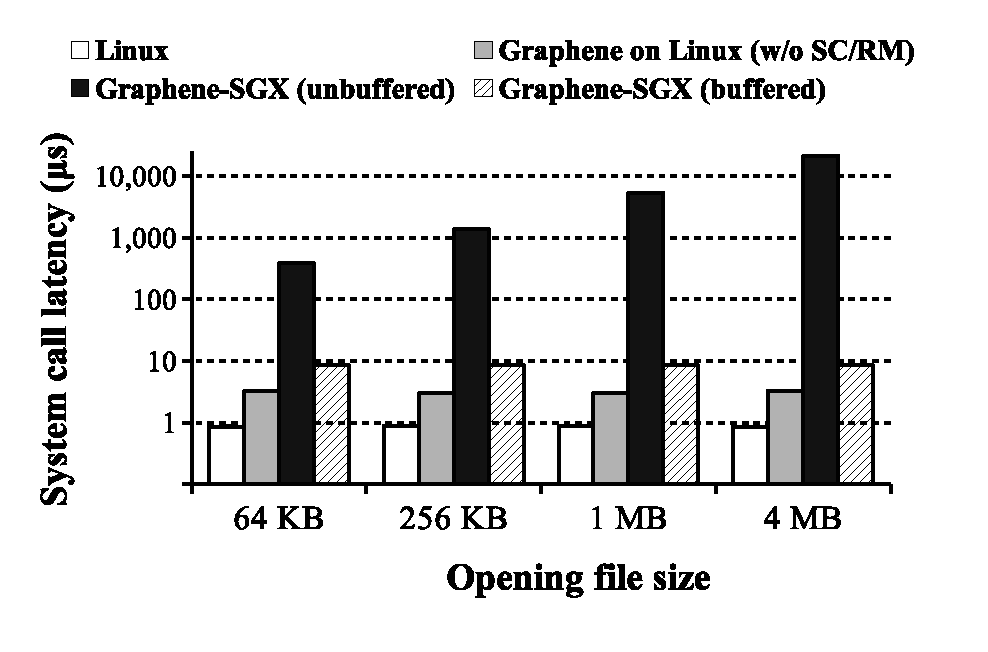
\includegraphics[width=\linewidth]{sgx/open-latency}\\
{\bf (a) Open a file}
\end{minipage}
\begin{minipage}{.3\textwidth}
\centering
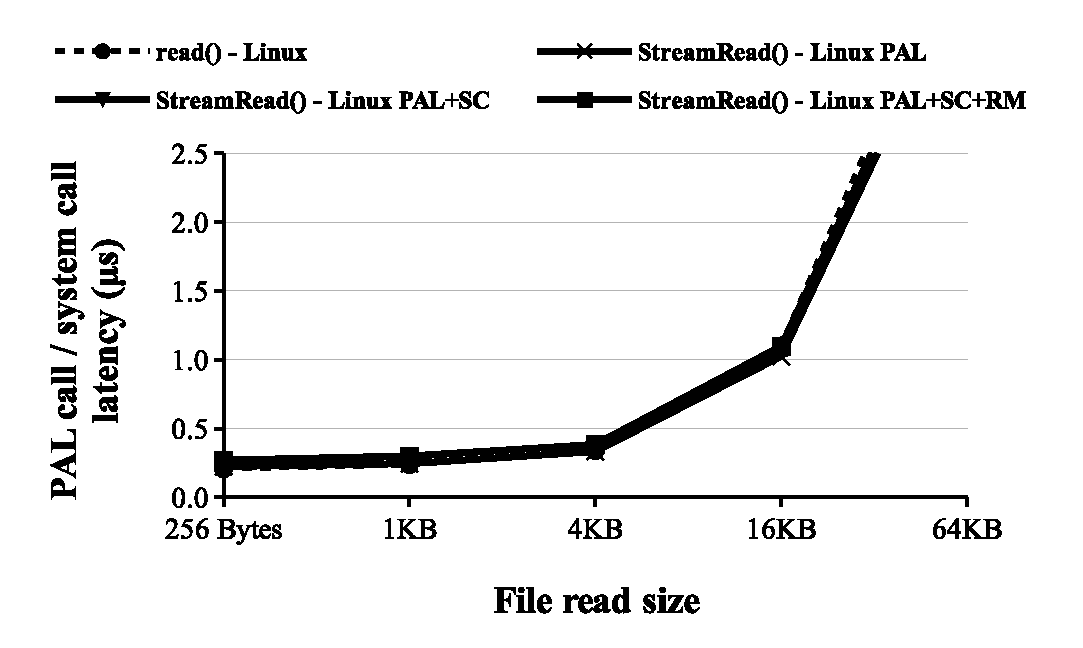
\includegraphics[width=\linewidth]{sgx/read-latency}\\
{\bf (b) Read a file}
\end{minipage}
\begin{minipage}{.3\textwidth}
\centering
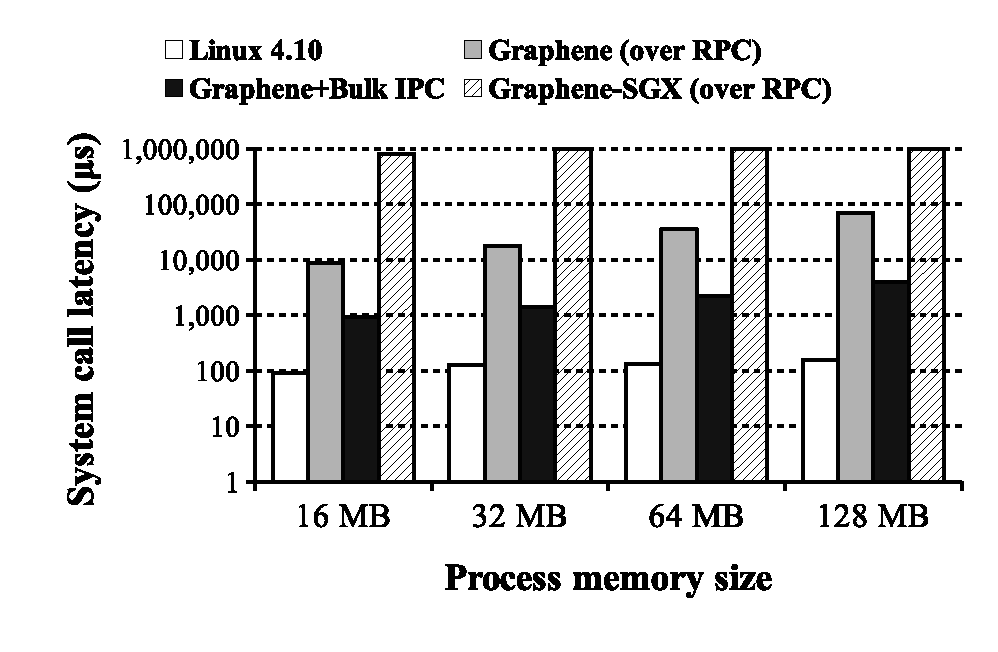
\includegraphics[width=\linewidth]{sgx/fork-latency}\\
{\bf (c) Fork a process}
\end{minipage}

\caption{Latency of some expensive system calls in \graphenesgx{}, including opening and reading a secured (authenticated) file, and forking a new process. The results are compared with native Linux and \graphene{}.}
\label{fig:syscall}
\end{figure*}


\subsection{Performance Overhead Analysis}


In this section we evaluate a few system operations that are heavily impacted by the \graphenesgx{} design.
%To shield dynamic loading and process creation,
%\graphenesgx{} uses computationally-expensive cryptographic techniques \fixmedp{more specific?} to verify enclave inputs.
% under the circumstance that the host OS cannot be trusted.
%As a trade-off to the security, the performance will be affected
%by additional cryptographic computation.
We measure the \syscall{open}, \syscall{read}, and \syscall{fork} system calls
using LMbench 2.5~\cite{McVoy:lmbench}.
A primary source of the overheads on these system calls is the cost of shielding applications, with run-time checks on the inputs.
Cryptographic techniques are used to: (1) validate the file against the secure hash, at \syscall{open}, (2) check the file chunks against the Merkle tree, at \syscall{read}, and (3) establish a TLS connection over inter-enclave RPC, at \syscall{fork}.
%opening a integrity-sensitive file for the first time, 
% or using cryptographic techniques, such as secure hashing, to verify the inputs.
% microbenchmarking specific system calls: 
% system calls,
%with different application settings.
%The microbenchmark is part of the LMBench 2.5 test suite
%\fixmedp{maybe merge this in the above paragraph, which feels a little coy}
%For instance, in order to shield dynamic loading, \graphenesgx{} checks each binary file against the secure hashes in the manifest,
%when the file is opened for the first time---after the whole file is copied into the enclave.
%\fixmedp{This happens after they are copied into enclave, memory right?}
%The verification happens when opening the file for the first time (often by the 
%After \graphenesgx{} validates the file, we generate a series of hashes of the file in chunks, as a merkle tree.
%to prevent verifying the whole file again when later randomly reading a part of the file.
%\fixmedp{So is this for the case when a file is swapped out?  I'm confused here - some details are missing}
%The latency of opening and reading an authenticated file in \graphenesgx{} is dominated by SHA256 and SHA512 calculation.
The remaining overheads contribute to exiting the enclave for host system calls, and bringing memory into the EPC (enclave page cache) or decrypting 
memory on a last-level cache miss. %and later the cache where the memory is decrypted by the CPU.


Figure~\ref{fig:syscall}(a)
shows the overhead for authenticating files in \syscall{open}.
\fixme{change overhead to latency}
Depending on the file size, the latency of \syscall{open} on \graphenesgx{} is 383$\mu$s (64KB file) to 21ms (4MB file), whereas on Linux, the latency is constant at 0.85$\mu$s.
We note that this is where enclaves are at a disadvantage, as \syscall{open} 
normally does not need to read file content; whereas here \graphenesgx{} uses \syscall{open}
as a point at which to validate file content.
For a subsequent \syscall{open}, when the Merkle tree is already generated, the overhead of simply exiting enclave for \syscall{open}, and searching the file list in the manifest, is about 9$\times$.
%\fixmedp{why?}


One might be able to optimize further for cases where only part of a file is accessed
with incremental hashing.  However, in the common case where nearly all of the file is accessed,
these costs are difficult to avoid when host file system is untrusted.
Another opportunity 
is to create the Merkle tree offline, when the manifest is created.
%\fixmedp{I think the second idea has legs...}


%This is an inevitable cost, because normal \funcname{open} on trusted OSes
%need not to access file content.
%After verifying the file, \graphenesgx{} buffers the chunk hash values, to skip whole-file verification when the file is reopened.

Figure~\ref{fig:syscall}(b)
shows the overhead for authenticating files in \syscall{read}, which 
is lower than \syscall{open}.
Since the whole file has been verified at \syscall{open}, the sequential \syscall{read} only verifies the chunks of files it is reading from untrusted memory.
%Reads from data cached in enclave memory are cheaper.  %\fixmedp{right? can we say how much cheaper?  Maybe add separate bars for both cases?}
% Therefore, \syscall{read} is actually much cheaper than \syscall{open}.
Depending on the size of blocks being read, the latency on \graphenesgx{} is 0.5$\mu$s (64-byte \syscall{read}) to 16.9$\mu$s (4KB \syscall{read}). The latency of \syscall{read} on Linux is \roughly{}0.1$\mu$s for any block size below 4KB.
If the file is not authenticated,
\graphenesgx{} only copies the file contents into the buffer, and the overhead reduces to 48\% (64-byte \syscall{read}) to 83\% (4KB \syscall{read}).
\fixmedp{Consider doing larger buffers, say up to 64k or even 4 MB}

%\fixmedp{In the legend for 7b, unsecure should be insecure}


Figure~\ref{fig:syscall}(c) shows the overhead of forking a process.
As described in \ref{sec:multiproc}, the latency of \syscall{fork} in \graphenesgx{} is affected by three factors:
creation of a new enclave, local attestation of the integrity, and duplicating the process state over an encrypted RPC stream.
Combining these factors, \syscall{fork} is one of the most expensive calls in \graphenesgx{}.
%, but at least it is supported natively on the current hardware.
The default enclave size is 256MB.
%which takes \roughly{}0.5s to create. 
Our evaluation shows that the latency of forking a process is around 0.8s (16MB process) to 2.7s (128MB process), but can be more expensive if the parent process uses more memory.
The trend matches the performance of \graphene{} without the bulk IPC optimization.
\fixmedp{If you want, some thoughts on how this might be improved in the future would be nice...  One good suggestion is recycling enclaves, or pre-forking so measurements can be done in parallel}
%Due to the overhead on \funcname{fork}, \graphenesgx{} is not suitable for fork-intensive workloads like Bash scripts
%if performance is critical.

\fixme{talk about a limitation of improving fork. check this.}
One way to further optimize \syscall{fork} is to reduce or avoid enclave creation time; one can potentially pre-launch a child enclave, and then migrate the process contents later when \syscall{fork} is called.
There might be another opportunity to improve the latency of process migration,
if copy-on-write sharing of enclave pages can be supported in future generations of SGX.
%Unfortunately, sending the process contents is difficult to avoid in \syscall{fork},
%as SGX disallows sharing enclave memory between multiple enclaves.

%\fixmedp{I assume 5.4 isn't done yet}



\subsection{TCB Size and Shielded Functionality}

In this section we measure the increase in TCB size of \graphenesgx{},
%in lines of code, 
as well as 
%compare the TCB size increased by \graphenesgx{} to an unmodified application, in lines of code, and 
the OS functionality shielded by the framework.
We compare to \scone{} and \panoply{}, using
%For SCONE and Panoply, we use 
numbers reported in their papers. 
%The conventional One generally assumes 
A smaller TCB is generally easier to review or possibly verify,
and is assumed to have fewer vulnerabilities.
%more implies lower burden for code review or formal verification, and less risk of writing exploitable code.
%For instance, Panoply argues that, because its use cases are typically smaller than 20kLoC, including both the application logic and Panoply itself, it is within the realm of future, automated verification~\cite{shinde17panoply}.

\fixmedp{Reviewer B asks for memory footprint, which isn't a bad idea}

\begin{table}
\footnotesize
\centering
\bgroup
\def\arraystretch{1.2}
\setlength{\tabcolsep}{0.5em}
\begin{tabular}{>{\raggedright\arraybackslash}p{9em}>{\raggedleft\arraybackslash\bf}p{7em}>{\raggedleft\arraybackslash}p{4.25em}>{\raggedleft\arraybackslash}p{4.25em}}
Components                    & \graphenesgx{}  & \scone{}     & \panoply{}  \\
\hline
libc (ld, libm, pthread)      &  1,292 &   88 & --      \\
                              & (glibc-2.19) & (musl)   &          \\
Library OS                    &     34 &  --      & --     \\
PAL / OS Shield               &     22 &   99 & 10  \\
\hline
Total                         &  1,348 &  187 & 10  \\
\hline
\end{tabular}
\egroup
\caption{TCB size (in thousands of lines of code) of \graphenesgx{}, \scone{}, and \panoply{}.}
\label{tab:tcb-size}
\end{table}

Table~\ref{tab:tcb-size} lists the lines of code in each components within the TCB of \graphenesgx{}, \scone{}, and \panoply{}.
By comparing the total TCB size, \graphenesgx{} is 9$\times{}$ larger than \scone{}, and 134$\times{}$ larger than \panoply{}.
However, the primary difference is the selection of libc: 
for maximum compatibility, \graphene{} uses glibc.
\scone{} uses the smaller musl libc, which lacks some features of glibc.
%it would be easy to use the smaller, and incomplete, musl libc.
%SCONE uses 
% Linux applications, \graphenesgx{} chooses to use a minimally-modified glibc, whereas SCONE uses the much more lightweight musl and 
\panoply{} excludes libc from its TCB,
% \fixmedp{what is their rationale, again? Check this}
to fit into the range of automated formal verification,
as they shield at the libc interface.
In principle, \graphene{} could easily support musl as well as glibc for applications
that do not need the additional features of glibc.
We also see the benefit of removing unused code from 
libraries, especially in an unsafe language,
similar to the approach taken in unikernels~\cite{unikernels}.
On balance, 
this choice of libc implementation is largely orthogonal to the issue
of how general-purpose the shields are.

%We argue that the choice of libc is orthogonal to the design of \graphenesgx{}; one can statically compile the applications against musl or glibc if TCB size is a concern, or given plenty of time, trim the libc functionality to bare minimum. 

If we focus on the TCB size of the library OS and the shields, 
\graphenesgx{} is 
%library OS and PAL in \graphenesgx{}, with the shielding layer of SCONE, we are 
44\% smaller than \scone{}. 
We cannot analyze the size of \scone{} because it is closed source.
%, although
%we suspect
%Although it is unclear what is in the implementation of SCONE, because it is not yet open-sourced, we believe the largest portion of their TCB contributes to the cryptography library.
\panoply{} has a smaller TCB in its shield, but within the same order of magnitude.
Panoply only shields 91 out of 256 supported POSIX functions; for context, POSIX 1003.1 defines 1,191 APIs~\cite{POSIX1003-1-2008}.
%out of 256 currently supported by \panoply{} \fixmedp{The better number is how many total functions in POSIX}.

All three of these compatibility layers or shields are within the same
order of magnitude in code size, and the differences are likely 
correlated with different ranges of supported functionality.
A recent study indicates that only order-of-magnitude differences in code
size correlate with reported CVE vulnerabilities; within the same order-of-magnitude,
the data is inconclusive that there is a meaningful difference in risk~\cite{security-metric}.
Thus, increased generality does not necessarily come with 
increased risk. % is not a clear relationship between risk 

% data only correlates
%with differences in code size when 

%Besides the choice of libc, we argue that the TCB size of a library OS or a shim shielding layer is actually correlated with the functionality that it supports or shields. Because none of the three frameworks have completely shielded the whole Linux system call table or POSIX, it is unclear how much code has to be added in the future. \graphenesgx{} also shows that one can always engineer a library OS with a small TCB, if most code is not reused from a monolithic OS kernel like Windows or Linux.
%A recent study of the CVE database also points out that having a larger TCB does not necessarily indicate more vulnerabilities, even when the difference is more than two order-of-magnitude. 



\input{apistudy}

\makeatletter
\def\input@path{{}}
\makeatother
\graphicspath{{}}
\section{Summary}



The Linux PAL successfully leverages a limited subset of Linux system calls,
to implement the whole PAL ABI for running a
full-featured \libos{}.
\Thehostabi{} separates the development of a host OS or hypervisor
from the complexity of emulating a sufficiently-compatible
Linux kernel.
The chapter shows that most calls in \thehostabi{}
can be directly translated to similar system calls on a Linux host kernel.
Only a few \hostapis{}, such as process creation and inter-thread synchronization, require additional attention for developing an efficient implementation strategy.



The Linux PAL also enforces robust security isolation
between mutually-untrusting applications,
by placing applications in separate, VM-like sandboxes.
The security isolation on a Linux host is based on system call restriction using a \seccomp{} filter, and a trusted reference monitor. % for checking resource access.
Security isolation at the host interface
restricts an untrusted application to explore vulnerable execution paths
inside a Linux kernel.
A \seccomp{} filter 
enforce a fixed, minimal system call profile, regardless of bloated dependency of an application.
The reference monitor follows
simple, white-listed manifest rules listing 
all the authorized files and network addresses of an application,
using well-known semantics
such as AppArmor~\cite{apparmor} or iptable-like firewall rules~\cite{iptablesman}.
The reference monitor can further enforce dynamic, process-specific isolation by splitting a sandbox
to run a child \picoproc{} under more restricted
resource permissions.
\graphene{} on a Linux host can serve as a sandbox framework
with a reduced attack surface
upon the host kernel.









\makeatletter
\def\input@path{{}}
\makeatother
\graphicspath{{}}
